%*********************************
%Format telah disesuaikan sesuai *
%Panduan penulisan               *
%Disertasi Dan Tesis ITS         *
%*********************************
\documentclass[12pt, a4paper,twoside, bahasa]{report}
%\documentclass[12pt, a4paper,twoside]{report}

\title{Buku Tesis}
% Jika pakai windows untuk run
%    pertama kali dan error.
% Mohon cek miktex console jika 
%    compiler latex nya menggunakan miktex. 
%------------------------------
%%%%%%%%%%%%%%%%%%%%%%%%%%%%%%%%%%%%%%%%%%%%
% FILE INI JANGAN DI UBAH
%%%%%%%%%%%%%%%%%%%%%%%%%%%%%%%%%%%%%%%%%%%%
%\usepackage[indonesian]{babel}
\usepackage[american]{babel}
%\usepackage[indonesian]{babel}
\usepackage[table,xcdraw]{xcolor}


\usepackage[pdfauthor={Nur Afandi},bookmarksnumbered,pdfborder={0 0 0}]{hyperref}
\usepackage[ruled,lined,commentsnumbered,linesnumbered]{algorithm2e}
\usepackage[utf8]{inputenc}
\usepackage{graphicx}
\usepackage{lipsum}  
\usepackage{hyphenat}
\usepackage{rotating}
\usepackage{booktabs}
\usepackage{lscape}
%\usepackage{algpseudocode}
\usepackage[ruled,lined,commentsnumbered,linesnumbered]{algorithm2e}
\usepackage{algpseudocode}
\usepackage{makeidx}
\usepackage{rotating}
\makeindex
\usepackage{epsfig}
\usepackage{subfig}
\usepackage{pdflscape}
\usepackage[doublespacing]{setspace}
\setstretch{1.5}
\usepackage{type1cm}
\usepackage{longtable}
\usepackage{lscape}
\usepackage{lettrine}
\usepackage{hyperref}
\usepackage[pageref]{backref}
\usepackage{multirow}
\usepackage[table,xcdraw]{xcolor}
\usepackage{eso-pic}
\newcommand\BackgroundIm{
	\put(0,0){
		\parbox[b][\paperheight]{\paperwidth}{%
			\vfill
			\centering
			\includegraphics[height=\paperheight,
			keepaspectratio]{./lib/background.png}%
			\vfill
}}}

\usepackage{fancyhdr} % Untuk pengaturan header dan footer yang lebih kompleks
\usepackage{etoolbox} % Untuk melakukan perubahan (patch) command internal LaTeX
\usepackage{url}
\usepackage{longtable}
\usepackage{float}
\usepackage{morefloats}
\floatstyle{boxed}
\newfloat{program}{thp}{lop}
\floatname{program}{Program}
\usepackage[fleqn]{amsmath}
\usepackage{nccmath}
\usepackage{enumitem}
\usepackage{ulem}
\usepackage[final]{pdfpages}
\usepackage{titlesec}
\usepackage{array}
\usepackage{multicol}
\usepackage{listings}
\usepackage{wrapfig}
\usepackage{array,tabularx}
\usepackage{lscape}
\usepackage{longtable}
\usepackage{caption}
\usepackage[export]{adjustbox}
\usepackage{ragged2e}
\usepackage{epsfig}
\usepackage{subfig}
\usepackage[top=35mm,left=40mm,right=30mm,bottom=30mm]{geometry}
\usepackage{pdflscape}
\usepackage[doublespacing]{setspace}
\setstretch{1.5}
\usepackage{type1cm}
\usepackage{lettrine}
\usepackage{hyperref}
\usepackage[pageref]{backref}
\usepackage{multirow}
\usepackage[table,xcdraw]{xcolor}
\usepackage{fancyhdr} % Untuk pengaturan header dan footer yang lebih kompleks
\usepackage{etoolbox} % Untuk melakukan perubahan (patch) command internal LaTeX
\usepackage{url}
\usepackage{longtable}
\usepackage{float}
\usepackage{morefloats}
\floatstyle{boxed}
\newfloat{program}{thp}{lop}
\floatname{program}{Program}
\usepackage[fleqn]{amsmath}
\usepackage{enumitem}
\usepackage{ulem}
\usepackage[final]{pdfpages}
\usepackage{titlesec}
\usepackage{array}
\usepackage{multicol}
\usepackage{listings}
\usepackage{wrapfig}
\usepackage{array,tabularx}
\usepackage{longtable}
\usepackage{caption}
%\usepackage{natbib}
%\usepackage[numbers]{natbib}
\usepackage[numbers]{natbib}

%\usepackage[sorting=none]{biblatex}

%square,sort,comma,numbers

%\renewcommand{\uline}[1]{\textit{#1}}
%\bibliographystyle{apalike}
\usepackage[export]{adjustbox}
\usepackage{ragged2e}
\usepackage[utf8]{inputenc}
\usepackage{afterpage}
\usepackage{lipsum}
%\usepackage{cite}
% More tidy url
%\usepackage{url}
%\usepackage{breakurl}
%\def\UrlBreaks{\do\/\do-\do.}

% Set paper size and margin
\usepackage{geometry}
\geometry{
	a4paper,
	left=40mm,
	top=35mm,
	right=30mm,
	bottom=30mm,
}

\usepackage{nomencl}
\makenomenclature

% untuk Cover
\newenvironment{FontCover}{\fontfamily{phv}\selectfont}{\par}
% untuk Lembar Pengesahan
\newenvironment{Kondisi}
{\par\vspace{\abovedisplayskip}\noindent
	\tabularx{\columnwidth}{>{$}l<{$} @{${}:{}$} >{\raggedright\arraybackslash}X}}
{\endtabularx\par\vspace{\belowdisplayskip}}
\newenvironment{Kondisi2}
{\par\vspace{\abovedisplayskip}\noindent
	\tabularx{\columnwidth}{>{$}l<{$} @{${}:{}$} >{\raggedright\arraybackslash}X}}
{\endtabularx\par\vspace{\belowdisplayskip}}
% Line spacing
\linespread{1.5}

% fix titlesec bug
\makeatletter
\patchcmd{\ttlh@hang}{\parindent\z@}{\parindent\z@\leavevmode}{}{}
\patchcmd{\ttlh@hang}{\noindent}{}{}{}
\makeatother

% Pengaturan format Chapter dan Section
\titleformat{\chapter}[display]{\bfseries\Large}{BAB \centering\thechapter}{0ex}{\vspace{0ex}\centering}[\vspace{3ex}]
\titlespacing*{\chapter}{0pt}{-4ex}{0pt}
\titleformat{\section}{\bfseries\normalsize}{\MakeUppercase{\thesection}}{1ex}{}
\titleformat{\subsection}{\normalsize\bfseries}
\titleformat{\subsubsection}{\normalsize\bfseries}

\titlespacing{\section}{0pt}{0pt}{1ex}
\titlespacing{\subsection}{0pt}{0pt}{1ex}
\titlespacing{\subsubsection}{0pt}{0pt}{1ex} 

% Keterangan rumus
\newenvironment{conditions}
{\par\vspace{\abovedisplayskip}\noindent
	\tabularx{\columnwidth}{>{$}l<{$} @{${}={}$} >{\raggedright\arraybackslash}X}}
{\endtabularx\par\vspace{\belowdisplayskip}}

% Caption label bold
\usepackage[labelfont=bf]{caption}
\captionsetup{labelfont=bf}

% Jarak caption dengan obyek
\captionsetup[figure]{font=small,skip=15pt}
\captionsetup[table]{font=small,skip=15pt}


\DeclareCaptionLabelSeparator{none}{}
\captionsetup{labelsep=period}
% Caption nama
\renewcommand{\figurename}{Gambar}
\renewcommand{\tablename}{Tabel}
\renewcommand{\lstlistingname}{Kode}

% Cek nomor halaman
\usepackage{changepage}

% Cek spelling
\usepackage{lipsum}
\setcounter{secnumdepth}{5}
\hyphenation{meng-gerak-kan mem-per-kenal-kan pe-ri-la-ku di-je-las-kan mem-bu-tuh-kan me-ne-rap-kan}

% Definisi untuk "halaman sengaja dikosongkan"
\def\kosong{
	\vspace*{\fill}
	\begin{center}\textit{This page is intentionally left blank}\end{center}
	\vfill
}

% Halaman sengaja dikosongkan
\patchcmd{\cleardoublepage}{\hbox{}}{\kosong}{}{}
% Untuk citation
%\newcommand{\tab}[1]{\hspace{.2\textwidth}\rlap{#1}}
\renewcommand*{\backreflastsep}{, }
\renewcommand*{\backreftwosep}{, }
\renewcommand*{\backref}[1]{}
%\renewcommand*{\backrefalt}[4]{
%	\ifcase #1
%	No citations.
%	\or
%	(Dikutip pada halaman #2).
%	\else
%	(Dikutip pada halaman #2).
%	\fi
%}
% Pengaturan penomoran halaman menggunakan package fancyhdr
\fancyhf{} 								% Mengosongkan header dan footer
\renewcommand{\headrulewidth}{0pt} 		% Menghapus garis horizontal pada header
\pagestyle{fancy} 						% Mengubah pagestyle dokumen menjadi fancy
\fancyfoot[CE,CO]{\thepage}				% Footer kanan pada hal. ganjil dan sebaliknya
%\patchcmd{\chapter}{plain}{fancy}{}{} 	% Mengubah pagestyle pada chapter menjadi fancy
\patchcmd{\chapter}{empty}{plain}{}{}
\usepackage{ifthen}
\newboolean{PembimbingDua}
\setboolean{PembimbingDua}{false}
\newboolean{bThesis}
\setboolean{bThesis}{true}

%\newcommand{\Tesis}
%{	\setboolean{bThesis}{true}
%}



\newboolean{PembimbingTiga}
\setboolean{PembimbingTiga}{false}

\newboolean{PengujiTiga}
\setboolean{PengujiTiga}{false}

\newboolean{PengujiEmpat}
\setboolean{PengujiEmpat}{false}

\newboolean{Nomenklatur}
\setboolean{Nomenklatur}{false}

\newboolean{bDoktor}
\setboolean{bDoktor}{false}
\newboolean{bMaster}
\setboolean{bMaster}{false}

\renewcommand{\em}[1]{\textit{#1}}
\renewcommand{\emph}[1]{\textit{#1}}

\newcommand{\Mahasiswa}[2]{
	\newcommand{\NamaMahasiswa}{#1}
	\newcommand{\NrpMahasiswa}{#2}
}
\newcommand{\PembimbingSatu}[2]
{
	\newcommand{\PbSatu}{#1}
	\newcommand{\NipPbSatu}{#2}
}
\newcommand{\PembimbingDua}[2]{
	\setboolean{PembimbingDua}{true}
	\newcommand{\PbDua}{#1}
	\newcommand{\NipPbDua}{#2}
}

\newcommand{\PembimbingTiga}[2]{
	\setboolean{PembimbingTiga}{true}
	\newcommand{\PbTiga}{#1}
	\newcommand{\NipPbTiga}{#2}
}

\newcommand{\PengujiSatu}[2]
{
	\newcommand{\PjSatu}{#1}
	\newcommand{\NipPjSatu}{#2}
}
\newcommand{\PengujiDua}[2]
{	\newcommand{\PjDua}{#1}
	\newcommand{\NipPjDua}{#2}
}
\newcommand{\PengujiTiga}[2]
{
\setboolean{PengujiTiga}{true}
\newcommand{\PjTiga}{#1}
\newcommand{\NipPjTiga}{#2}
}

\newcommand{\PengujiEmpat}[2]
{
\setboolean{PengujiEmpat}{true}
	\newcommand{\PjEmpat}{#1}
	\newcommand{\NipPjEmpat}{#2}
}
\newcommand{\KaDep}[2]
{
	\newcommand{\NmKaDep}{#1}
	\newcommand{\NipKaDep}{#2}
}
\newcommand{\CoverFooter}[1]
{\newcommand{\bdk}{#1}
}
\newcommand{\Judul}[1]
{
	\newcommand{\JdTesis}{#1}
}
\newcommand{\TanggalUjian}[1]
{
	\newcommand{\TglUjian}{#1}
}
\newcommand{\PeriodeWisuda}[1]
{
	\newcommand{\PerWisuda}{#1}
}

\newcommand{\Fakultas}[1]
{
	\newcommand{\fak}{#1}
}
\newcommand{\BeltFakultas}[1]
{
	\newcommand{\bbelt}{#1}
}
\newcommand{\Departemen}[1]
{
	\newcommand{\Dep}{#1}
}
\newcommand{\ggGelar}{xxxx}
\newcommand{\pPengesahan}{xxxxxxxx}

\newcommand{\Gelar}[1]
{
	\renewcommand{\ggGelar}{#1}
}

\newcommand{\tsss}{Disertasi disusun untuk memenuhi salah satu syarat memperoleh gelar}

\newcommand{\Disertasi}[1]
{\renewcommand{\tsss}{Disertasi disusun untuk memenuhi salah satu syarat memperoleh gelar}
	\renewcommand{\pPengesahan}{LEMBAR PENGESAHAN DISERTASI}
	\renewcommand{\ggGelar}{#1}
	 \setboolean{bMaster}{false}
	 \setboolean{bThesis}{true}
}

\newcommand{\prop}{PROPOSAL DISERTASI}
\newcommand{\ProposalDisertasi}
{	\renewcommand{\prop}{PROPOSAL DISERTASI}
	\setboolean{bMaster}{false}
	\setboolean{bThesis}{false}
}

\newcommand{\Tesis}[1]
{	
	\renewcommand{\tsss}{Tesis disusun untuk memenuhi salah satu syarat memperoleh gelar}
	\renewcommand{\pPengesahan}{LEMBAR PENGESAHAN TESIS}
    \setboolean{bMaster}{true}
    \setboolean{bThesis}{true}
    \renewcommand{\ggGelar}{#1}

}

\newcommand{\ProposalTesis}
{	\setboolean{bMaster}{true}
	\renewcommand{\prop}{THESIS PROPOSAL}
	\setboolean{bThesis}{false}
}


\newboolean{JudulTesisEng}
\setboolean{JudulTesisEng}{true}

\newcommand{\JudulEng}[1]
{
	\setboolean{JudulTesisEng}{true}
	\newcommand{\JdTesisEng}{#1}
}

\newcommand{\Kode}[1]
{\newcommand{\Kodekk}{#1}
}

\newcommand{\TempatUjian}[1]
{
	\newcommand{\bTempatUjian}{#1}
}

\newcommand{\HariUjian}[1]
{
	\newcommand{\bHariUjian}{#1}
}

\newcommand{\DaftarRiwayatHidup}{
\addcontentsline{toc}{chapter}{Biodata Penulis}
\titlespacing*{\chapter}{0pt}{0ex}{5ex}
\appendix
\chapter*{AUTHOR BIODATA}
%*********************************
% Photo Section
\begin{center}
    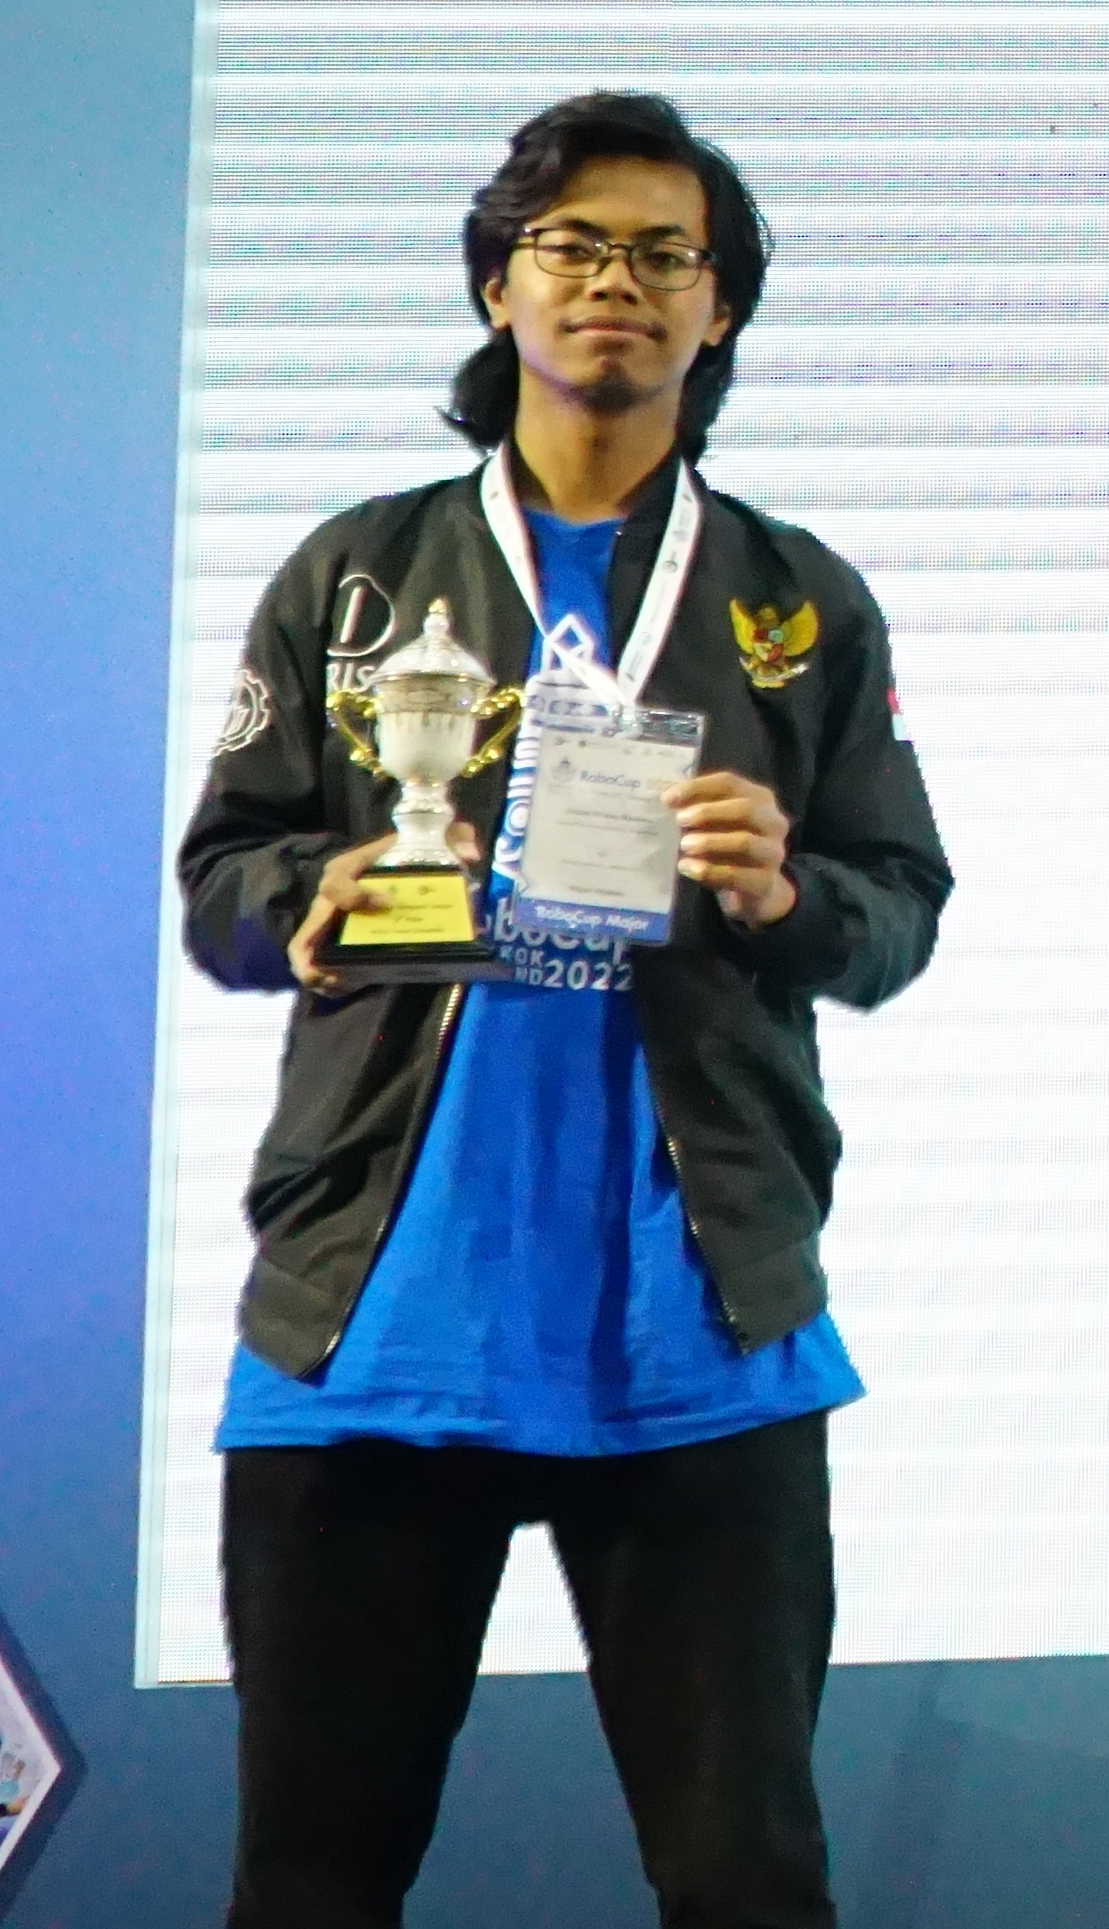
\includegraphics[height=0.2\textheight]{../ubah/Foto.jpg}
\end{center}
%*********************************

\section*{Personal Information}
\begin{tabular}{p{3cm}cp{9cm}}
    Name             & :& Azzam Widan Maulana \\
    Place of Birth   & :& Jember \\
    Date of Birth    & :& June 4, 2002 \\
    Address          & :& Arif Rahman Hakim Street No. 14A, Keputih, Sukolilo, Surabaya \\
\end{tabular}

\section*{Educational Background}
\begin{tabular}{p{3cm}cp{9cm}}
    2024–Present   & :& Master's Program (M.Sc.), Department of Electrical Engineering, Faculty of Intelligent Electrical and Informatics Technology, Institut Teknologi Sepuluh Nopember (ITS) \\
    &&\\
    2020–2024  & :& Bachelor Program (B.Eng.), Department of Computer Engineering, Faculty of Intelligent Electrical and Informatics Technology, Institut Teknologi Sepuluh Nopember (ITS) \\
    &&\\
    2017–2020  & :& SMAN 1 Jember \\
    &&\\
    2014–2017  & :& SMPN 3 Jember \\
    &&\\
    2008–2014  & :& SDN Kaliwates 2 Jember \\
    &&\\
    2006–2008  & :& TK Miftahul Ulum Kaliwates Jember \\
\end{tabular}

\section*{List of Publications}
\begin{enumerate}
    \item Muhtadin, A. W. Maulana, R. Dikairono and A. Zaini, "Omnivision Calibration on Mobile Robot Using Machine Learning," \textit{2024 International Conference on Computer Engineering, Network, and Intelligent Multimedia (CENIM)}, Surabaya, Indonesia, 2024, pp. 1–8, doi: 10.1109/CENIM64038.2024.10882712.
\end{enumerate}

\section*{Research History}
\begin{enumerate}
    \item Multicast Communication System on IRIS Robot 2022
    \item Natural Ball Handling System on IRIS Robot 2022
    \item Omnivision Camera Calibration on Mobile Robot Using Machine Learning 2023
    \item Robot Positioning System Using Gaussian Model on IRIS Robot 2023
    \item Empty Goal Detection System Using Omnivision Camera on IRIS Robot 2023
    \item Content Management System and User Interface for RAISA ITS Robot 2024
    \item Custom Operating System for Autonomous Vehicle and IRIS Robot 2024
    \item Empty Goal Detection System Using Stereo Depth Camera on IRIS Robot 2024
    \item Ball Detection System Using Spatial Image Classification on IRIS Robot 2024
    \item Hardware Communication System Using Layer 2 Communication for Autonomous Vehicle and IRIS Robot 2024
    \item Hardware Communication System Using CAN-bus for Autonomous Vehicle and IRIS Robot 2024
    \item End to End Machine Learning System for Autonomous Vehicle 2025
    \item Fleet Management System for AMR (Autonomous Mobile Robot) 2025
\end{enumerate}

\section*{Other Background}
Before venturing into the world of robotics and programming, the author was involved in music. As a musician, he mastered various musical instruments such as guitar, bass, and keyboard. In addition to playing instruments, he was also active in the field of mixing and mastering. His hobby of signal processing sparked an interest in learning how computers process signals. This passion led him to pursue a degree in Computer Engineering at ITS. Moreover, he delved into robotics to understand how computers and hardware operate, enabling him to perform advanced digital signal processing techniques.

\cleardoublepage}


\newcommand{\DaftarPustaka}{%\\renewcommand\bibname{Daftar Pustaka}
%\\addcontentsline{toc}{chapter}{\bibname}
%\\titlespacing*{\chapter}{0pt}{0ex}{5ex}
%\\appendix
%\%\bibliographystyle{apalike}
%\%\bibliographystyle{ieetr}
%\%\bibliographystyle{IEEEtranN}
%\\bibliographystyle{plainnat}
%\\bibliography{./ubah/pustaka}
%\\cleardoublepage
%\gdef \bibname{Daftar Pustaka}
\renewcommand \bibname {Bibliography}
\addcontentsline{toc}{chapter}{\bibname}
\titlespacing*{\chapter}{0pt}{0ex}{5ex}
\appendix
%\bibliographystyle{IEEEtranN}
% \bibliographystyle{IEEEtran} % ku ganti
\bibliographystyle{plain} % ku ganti
\bibliography{IEEEabrv,../ubah/pustaka.bib}
%\bibliography{IEEEabrv,pustaka.bib}
%\bibliography{../ubah/pustaka.bib}
%\bibliography{library}
\cleardoublepage}

\tolerance=9999
\emergencystretch=10pt
\hyphenpenalty=10000
\exhyphenpenalty=100
\usepackage{placeins}



%************************************
% 1. JENIS BUKU
%    Pilih Salah Satu 
%************************************
%     \ProposalDisertasi
     \ProposalTesis 
%     \Tesis{Magister Teknik (MT)}
%\Disertasi{Doktor (Dr)}
%***************************

%\ProposalDisertasi
%\ProposalTesis 
%\Tesis{Magister Teknik (MT)}
%\Disertasi{Doktor (Dr)}


%*******************************
%2.  Tulislah Kode Yang Sesuai 
%*******************************
%\Kode{DISERTASI - EE186601}
%\Kode{TESIS - EE184401}
%\Kode{Proposal Tesis}
\Kode{Thesis Proposal}
%\Kode{Proposal Disertasi}
%*******************************

%*******************************
%  3. Judul Proposal, Tesis atau 
%     Disertasi 
%     dipilih Salah Satu 
%-------------------------------
% Tulislah Judul Dalam Bahasa Indonesia
\Judul{AUTONOMOUS VEHICLE NAVIGATION SYSTEM USING MACHINE LEARNING AND GRAPH BASED SLAM}
% Tulislah Judul Dalam Bahasa Inggris
\JudulEng{AUTONOMOUS VEHICLE NAVIGATION SYSTEM USING MACHINE LEARNING AND GRAPH BASED SLAM}
%***********************************
% 4. Identitas Mahasiswa
% Format :\Mahasiswa{Nama}{Nrp}
%------------------------------------
\Mahasiswa{Azzam Wildan Maulana}{6022241101}
%************************************
% 5. Waktu Dan Ruang Ujian
%------------------------------------
%Tanggal Ujian 
\TanggalUjian{26 June 2025}
% Perioda wisuda  
%\PeriodeWisuda{September 2023} 
%Hari ujian dan Tempat Ujian 
\HariUjian{Thursday}
\TempatUjian{B211 Room}


%************************************
%6. Identitas Pembimbing 
%   Maximal Tiga Pembimbing
%   Format : \PembimbingXXX{Nama}{Nip}
%-----------------------------------
%\scalebox{.95}[1.0]{xxx}
\PembimbingSatu{Prof. Dr. Ir. Mauridhi Hery Purnomo, M.Eng.}{195809161986011001}
\PembimbingDua{Ahmad Zaini, S.T., M.Sc.}{197504192002121003}
\PembimbingTiga{Dr. Rudy Dikairono, S.T., M.T.}{198103252005011002}

%************************************
% 7. Identitas Penguji 
%     Maximal 4 penguji
%     Format : \PengujiXXX{Nama}{Nip}
%-------------------------
\PengujiSatu{Dr. Arief Kurniawan, S.T., M.T.}{197409072002121001}
\PengujiDua{Dr. Diah Puspito Wulandari, S.T., M.Sc.}{198012192005012001}
\PengujiTiga{Dr. Supeno Mardi Susiki Nugroho,S.T.,M.T.}{197003131995121001}
\PengujiEmpat{Dr.Eko Mulyanto Yuniarno}{132135221}
% \PengujiTiga{-}{-}
% \PengujiEmpat{-}{-}

%************************************
% 8. Identitas Fakultas ------------------------------------
\Fakultas{Fakultas Teknologi Elektro Dan Informatika Cerdas}
\BeltFakultas{BeltFte}
%************************************
% 9. Identitas Departement
%-----------------------------------
\Departemen{Teknik Elektro}

\KaDep{Dedet Candra Riawan, ST., M.Eng., Ph.D}{197311192000031001}
%***********************************
% 10. Footer Identitas Program Studi 
%  Pada Cover
%----------------------------------
\CoverFooter{\normalsize
MASTER PROGRAM\\
	DEPARTMENT OF ELECTRICAL ENGINEERING\\
	FACULTY OF INTELLIGENT ELECTRICAL AND\\
	INFORMATICS TECHNOLOGY\\
	INSTITUT TEKNOLOGI SEPULUH NOPEMBER\\
	SURABAYA\\
	2025}

%**********************************
%File Penting Yang Dapat di Edit:
%**********************************
%Abstrak :
%        ->\ubah\abstrak.tex
%Abstrak Bhs Inggris :
%        ->\ubah\abstrakEng.tex
%Kata Penggantar :
%        ->\ubah\pengantar.tex 
%Nomenklatur :
%        ->\ubah\Nomenklatur.tex
%Database Daftar Pustaka
%        ->\ubah\pustaka.bib
%DaftarRiwayatHidup 
%        ->\ubah\DaftarRiwayatHidup.tex
%----------------------------------
%**********************************
%Dokumen Utama
%----------------------------------
\begin{document}
%%%%%%%%%%%%%%%%%%%%%%%%%%%%%%%%%%%%%%%%%%%%
% FILE INI JANGAN DI UBAH ATAU MODIFIKASI
%%%%%%%%%%%%%%%%%%%%%%%%%%%%%%%%%%%%%%%%%%%%
\normalsize
\pagenumbering{roman}
\singlespacing
 \hyphenpenalty=1000
\tolerance=1000
\emergencystretch=2.5em
% Cover
%\addcontentsline{toc}{chapter}{Cover}
\begin{FontCover}
	\sffamily	
\thispagestyle{empty}
\begin{figure} [!t]
	
\includegraphics[keepaspectratio=true,scale=1,left]{./lib/LogoITS.png}
	\caption*{}
	\label{fig:LogoITS}
\end{figure}
\vspace{1ex}
%\noindent\makebox[\linewidth]{\rule{\paperwidth}{10pt}}
\makebox[\linewidth]{\includegraphics[keepaspectratio=true,width=\paperwidth]{./lib/\bbelt}}
\vspace{10ex}
\justify
\textbf{\Kodekk}
\vspace{1ex}
\justify
\Large
\begin{spacing}{1}
%Masukan Judul Tesis Disini
\flushleft
\textbf{\JdTesisEng}
\end{spacing}
\normalsize
\vfill
\justify

%\begin{spacing}{1}
\large
\MakeUppercase{\NamaMahasiswa}\\
NRP  \uppercase{\NrpMahasiswa}
\vspace{2ex}
\justify
\normalsize

\ifthenelse{\boolean{bMaster}}{\textbf{SUPERVISOR}}{\textbf{PROMOTOR}}\\
\PbSatu\\
\ifthenelse{\boolean{PembimbingDua}}{\ifthenelse{\boolean{bMaster}}{}{\\\textbf{Co.PROMOTOR\\}}}{}
\ifthenelse{\boolean{PembimbingDua}}{\PbDua\\}{}
\ifthenelse{\boolean{PembimbingTiga}}{\PbTiga\\}{}
 
\vfill
\justify
\bdk
\vspace{1ex}
%\rmfamily
\normalfont
\end{FontCover}
\newpage
\cleardoublepage
% Lembar pengesahan
\addcontentsline{toc}{chapter}{LEMBAR PENGESAHAN}

\ifthenelse{\boolean{bThesis}}
{ \AddToShipoutPicture*{\BackgroundIm}
\begin{center}

\Large\textbf{\pPengesahan}
%\Large\textbf{PROPOSAL TESIS}
\end{center}
\begin{center}
\tsss\\
\textbf{\ggGelar}\\
di\\
\textbf{Institut Teknologi Sepuluh Nopember}\\
\vspace{1ex}
Oleh:\\
\textbf{\NamaMahasiswa}\\ 
\textbf{NRP:\NrpMahasiswa}\\ 
\vspace{1ex}
Tanggal Ujian :\TglUjian\\
Periode Wisuda : \PerWisuda\\
\vspace{1ex}
\end{center}
\begin{center}
Disetujui oleh:\\
\textbf{Pembimbing}:
\end{center}
\begin{enumerate}
\item \PbSatu \hfill ...............................\\
NIP:\NipPbSatu \vfill
\ifthenelse{\boolean{PembimbingDua}}{\item \PbDua\hfill ...............................\\
NIP:\NipPbDua}\vfill
\ifthenelse{\boolean{PembimbingTiga}}{\item \PbTiga \hfill ...............................\\
	NIP:\NipPbTiga}{}
\end{enumerate}	
\begin{center}
	\textbf{Penguji}:
\end{center}
\begin{enumerate}
	\item \PjSatu \hfill ...............................\\
	NIP:\NipPjSatu
	\vfill
	\item \PjDua \hfill ...............................\\
	NIP:\NipPjDua\vfill
\ifthenelse{\boolean{PengujiTiga}}{
	\item \PjTiga \hfill ...............................\\NIP:\NipPjTiga\vfill}{}
\ifthenelse{\boolean{PengujiEmpat}}{
	\item \PjEmpat \hfill ...............................\\ NIP:\NipPjEmpat\vfill}{}
\end{enumerate}	
\vfill
\begin{center}
	Kepala Departemen \Dep \\
	 \fak\\
	\vspace{9ex}
	\underline{\NmKaDep}\\
	Nip:\NipKaDep
\end{center}
\newpage
}
{
\begin{center}
\textbf{VALIDITY SHEET\\
	\prop}\\    
\end{center}
\vspace{5ex}
\begin{tabular}{p{2cm} c p{8cm}}
Judul&:&\JdTesisEng\\
Oleh &:&\NamaMahasiswa\\
Nrp&:&\NrpMahasiswa
\end{tabular}
\vspace{5ex}
\begin{center}
\textbf{Has Been Presented On}
\end{center}
\begin{tabular}{p{2cm} c p{8cm}}
Day &:&\bHariUjian\\
Date &:&\TglUjian\\
Place&:&\bTempatUjian
\end{tabular}
\vspace{5ex}
%\scalebox{.95}[1.0]{\PjSatu}

\begin{tabular}{p{8cm} p{8cm} }
\textbf{Examiner}& \textbf{Supervisor}\\
\vspace{8ex}\hspace{-10ex}1. \PjSatu&
\vspace{8ex}\hspace{-8ex}1. \PbSatu \\
\hspace{-7ex}Nip :\NipPjSatu&
\hspace{-5ex}Nip :\NipPbSatu\\
\vspace{8ex}\hspace{-10ex}2. \PjDua&

\ifthenelse{\boolean{PembimbingDua}}
{\vspace{8ex}\hspace{-8ex}2. \PbDua}{} \\
\hspace{-7ex}Nip :\NipPjDua&
\ifthenelse{\boolean{PembimbingDua}}
{\hspace{-5ex}Nip :\NipPbDua}{}\\

% \ifthenelse{\boolean{PembimbingTiga}}
% {\vspace{8ex}\hspace{-8ex}3. \PbTiga}{} \\
% \ifthenelse{\boolean{PembimbingTiga}}
% {\hspace{-5ex}Nip :\NipPbTiga}{}\\

\vspace{8ex}\hspace{-10ex}3. \PjTiga&
\vspace{8ex}\hspace{-8ex}3. \PbTiga \\
\hspace{-7ex}Nip :\NipPjTiga&
\hspace{-5ex}Nip :\NipPbTiga\\

% \ifthenelse{\boolean{PengujiTiga}}
% {\vspace{8ex}\hspace{-10ex}}{}&
% \ifthenelse{\boolean{PengujiTiga}}
% {\hspace{-7ex}Nip :\NipPjTiga}{}&

% \ifthenelse{\boolean{PembimbingTiga}}
% {\vspace{8ex}\hspace{-8ex}3. \PbTiga}{} \\
% \hspace{-7ex}&
% \ifthenelse{\boolean{PembimbingTiga}}
% {\hspace{-5ex}Nip :\NipPbTiga}{}\\

% \ifthenelse{\boolean{PembimbingTiga}}
% {\vspace{8ex}\hspace{-8ex}3. \PbTiga}{} \\
% \ifthenelse{\boolean{PembimbingTiga}}
% {\hspace{-5ex}Nip :\NipPbTiga}{}\\


%\ifthenelse{\boolean{PengujiEmpat}}
%{\vspace{8ex}\hspace{-10ex}4. \PjTiga}{}& \\
%\ifthenelse{\boolean{PengujiEmpat}}
%{\hspace{-7ex}Nip :\NipPjEmpat}{}&\\
\end{tabular}
\newpage
}
\cleardoublepage

\ifthenelse{\boolean{bThesis}}
{
	\ifthenelse{\boolean{bMaster}}
	{
\chapter*{PERNYATAAN KEASLIAN TESIS}
\addcontentsline{toc}{chapter}{PERNYATAAN KEASLIAN TESIS}


\begin{spacing}{1.5}
	
	Dengan ini saya menyatakan bahwa isi keseluruhan Tesis saya dengan judul \textbf{\JdTesis} adalah benar-benar hasil karya intelektual mandiri, diselesaikan tanpa menggunakan bahan-bahan yang tidak diijinkan dan bukan merupakan karya pihak lain yang saya akui sebagai karya sendiri.
	
	Semua referensi yang dikutip maupun dirujuk telah ditulis secara lengkap pada daftar pustaka. Apabila ternyata pernyataan ini tidak benar, saya bersedia menerima sanksi sesuai peraturan yang berlaku.
	
	\hspace{30ex}Surabaya \today
	
	\vspace{10ex}
	
	\hspace{35ex}\underline{\NamaMahasiswa}
	
	\hspace{35ex}Nrp :\NrpMahasiswa
	
\end{spacing}
\cleardoublepage

}
{
	
	\chapter*{PERNYATAAN KEASLIAN DISERTASI}
	\addcontentsline{toc}{chapter}{PERNYATAAN KEASLIAN DISERTASI}
	
	\begin{spacing}{1.5}
		
		Dengan ini saya menyatakan bahwa isi keseluruhan Disertasi  saya dengan judul \textbf{\JdTesis} adalah benar-benar hasil karya intelektual mandiri, diselesaikan tanpa menggunakan bahan-bahan yang tidak diijinkan dan bukan merupakan karya pihak lain yang saya akui sebagai karya sendiri.
	
	Semua referensi yang dikutip maupun dirujuk telah ditulis secara lengkap pada daftar pustaka. Apabila ternyata pernyataan ini tidak benar, saya bersedia menerima sanksi sesuai peraturan yang berlaku.
	
	\hspace{30ex}Surabaya \today
	
	\vspace{10ex}
	
	\hspace{35ex}\underline{\NamaMahasiswa}
	
	\hspace{35ex}Nrp :\NrpMahasiswa
	
\end{spacing}
\cleardoublepage
}
}{}




% Kata pengantar
\newpage

\addcontentsline{toc}{chapter}{PREFACE}
\begin{center}
	\Large\textbf{PREFACE}
\end{center}
\vspace{2ex}
%Tulis kata pengantar di sini
Praise and gratitude to the presence of Allah SWT. for all His grace, the author was able to complete this research with the title \textbf{\JdTesis}. This research was written as a requirement for completing a master’s degree at the Department
of Electrical Engineering, Institut Teknologi Sepuluh Nopember.\\
The author also expresses great thanks to:
\begin{itemize}
	\item Parents and family for their encouragement and
	support during the author’s study.
	\item One girl who has always been there for the author, providing support and motivation during the author's study.
	\item My friends especially AWM and The Dangereous Family for supporting the author during the study.
\end{itemize}
\vspace{26pt}
\begin{flushright}
	\begin{tabular}[b]{c}
		Surabaya, June 2025
		\\
		\\
		\\
		The Author
	\end{tabular}
\end{flushright}

\cleardoublepage
\newpage
% Abstrak
%\begin{spacing}{1}
\begin{center}
		\large\textbf{\JdTesis}
	\end{center}
	\normalsize
	\begin{adjustwidth}{-0.2cm}{}
		\ifthenelse{\boolean{bMaster}}{
		
		\begin{tabular}{lcp{0.9\linewidth}}
		Nama Mahasiswa &:& \NamaMahasiswa\\
			NRP &:&\NrpMahasiswa\\
			Pembimbing &:& 1. \PbSatu\\
			\ifthenelse{\boolean{PembimbingDua}}{& & 2. \PbDua\\}{}
			
			\ifthenelse{\boolean{PembimbingTiga}}{& & 3. \PbTiga\\}{}
			
			
			
		\end{tabular}
	}{
	\begin{tabular}{lcp{0.7\linewidth}}
		Nama Mahasiswa &:& \NamaMahasiswa\\
		NRP &:&\NrpMahasiswa\\
		Promotor &:&  \PbSatu\\
		\ifthenelse{\boolean{PembimbingTiga}}{
		\ifthenelse{\boolean{PembimbingDua}}{Co. Promotor&: & 1. \PbDua\\}{}
		\ifthenelse{\boolean{PembimbingTiga}}{& & 2. \PbTiga\\}{}
	}
{
	\ifthenelse{\boolean{PembimbingDua}}{\hspace{5ex}Co. Promotor&: & \PbDua\\}{}
	
}
	\end{tabular}

}

	
	\end{adjustwidth}
	\vspace{2ex}
	\begin{center}
		\Large\textbf{ABSTRAK}
	\end{center}
	\vspace{1ex}	
%Tulis Abstrak disini
Explainable AI atau lebih banyak dikenal dengan sebutan XAI adalah sebuah metode untuk mengatasi permasalahan kotak hitam pada model AI. Yaitu sebuah permasalahan dimana sebuah model AI tidak transparan dan tidak bisa dijelaskan korelasi antara inpu-output nya. Pada riset ini dilakukan serangkaian percobaan untuk mengimplementasikan metode XAI pada model forecasting dan deteksi anomali. Persebaran panas pada boiler PLTU dijadikan sebagai studi kasus. Secara khusus, model yang diaplikasikan menggunakan arsitektur encoder-decoder, digunakan untuk melakukan forecasting temperature dari pipa-pipa reheater pada boiler dan untuk mendeteksi terjadinya anomali. Metode XAI yang digunakan berbasis pada feature importance. Output dari penelitian ini adalah informasi mengenai variabel input yang paling signifikan mempengaruhi output dari model AI.

%Tulis Kata Kunci disini
\vspace{2ex}
\textbf{Kata kunci }: XAI, Forecasting, Encoder-Decoder, Anomaly Detection
	
\end{spacing}
%\cleardoublepage
\ifthenelse{\boolean{JudulTesisEng}}
{
	\begin{spacing}{1}
\begin{center}
		\large\textbf{\JdTesisEng}
	\end{center}
	\normalsize
	\begin{adjustwidth}{-0.2cm}{}
		\begin{tabular}{lcp{0.9\linewidth}}
		By &:& \NamaMahasiswa\\
			Student Identity Number &:&\NrpMahasiswa\\
			Supervisor &:& 1. \PbSatu\\
			\ifthenelse{\boolean{PembimbingDua}}{& & 2. \PbDua\\}{}
			\ifthenelse{\boolean{PembimbingTiga}}{& & 3. \PbTiga\\}{}
		\end{tabular}
	\end{adjustwidth}
	\vspace{2ex}
	
	\begin{center}
		\Large\textbf{ABSTRACT}
	\end{center}
	\vspace{1ex}	
%Tulis Abstrak disini
Icar is an autonomous vehicle developed by Institut Teknologi Sepuluh Nopember (ITS) to autonomously navigate the campus environment. Its navigation system relies on pose estimation using sensor fusion between odometry and the Global Navigation Satellite System (GNSS). However, GNSS signals are prone to degradation in environments with obstacles such as tall buildings and trees, while odometry suffers from inaccuracies caused by wheel slippage, encoder drift, and inertial sensor errors. These limitations result in unreliable localization, potentially causing Icar to deviate from its designated trajectory.

To address these issues, this research proposes an enhanced navigation system by integrating a stereo depth camera and LIDAR. Road detection is performed using a semantic segmentation model based on deep learning, enabling Icar to distinguish road surfaces from non-road areas. Pose refinement is carried out using graph-based optimization within a SLAM framework, incorporating data from the depth camera and LIDAR processed via the Iterative Closest Point (ICP) algorithm. The proposed system improves localization robustness and offers a GNSS-independent alternative for safe and accurate autonomous navigation. The final system is expected to reduce dependency on GNSS and increase Icar's reliability in semi-structured or dynamic environments.

%Tulis Kata Kunci disini
\vspace{2ex}
\textbf{Keyword}: Autonomous vehicle, Icar, GNSS, Odometry, Pose Estimation, Stereo Depth Camera, Semantic Segmentation, SLAM, ICP, Graph-Based Optimization, Deep Learning
\end{spacing}
}{}
\cleardoublepage

% Daftar isi
\renewcommand*\contentsname{TABLE OF CONTENTS}
\titlespacing*{\chapter}{0pt}{0ex}{0ex}
\tableofcontents
\cleardoublepage
% Daftar gambar
\renewcommand*\listfigurename{LIST OF FIGURES}
\addcontentsline{toc}{chapter}{\listfigurename}
\titlespacing*{\chapter}{0pt}{0ex}{0ex}
\listoffigures
\cleardoublepage
% Daftar tabel
\renewcommand*\listtablename{LIST OF TABLES}
\addcontentsline{toc}{chapter}{\listtablename}
\titlespacing*{\chapter}{0pt}{0ex}{0ex}
\listoftables
\cleardoublepage
% Nomenklatur
\addcontentsline{toc}{chapter}{NOMENCLATURE} % kata pengantar
\begin{center}
\Large\textbf{NOMENKLATUR}
\end{center}
\vspace{1ex}

\begin{longtable}{p{5cm} p{10cm}}
	\textbf{Symbol / Acronym} & \textbf{Description} \\
	\hline
	$x_{\text{waypoint}}$ & X-coordinate of the waypoint from the predefined trajectory \\
	$y_{\text{waypoint}}$ & Y-coordinate of the waypoint from the predefined trajectory \\
	$x_{\text{position}}$ & Current X-coordinate of the vehicle \\
	$y_{\text{position}}$ & Current Y-coordinate of the vehicle \\
	$\theta_{\text{direction}}$ & Heading angle toward the waypoint \\
	$\theta_{\text{orientation}}$ & Current orientation of the vehicle \\
	$v_{\text{target}}$ & Target velocity of the vehicle \\
	$v_{\text{max}}$ & Maximum velocity allowed \\
	$\delta_{\text{target}}$ & Target steering angle based on bicycle model \\
	$L$ & Distance between the front and rear wheels \\
	$D_{\text{lookahead}}$ & Lookahead distance for path tracking \\
	\hline
	\textbf{GNSS} & Global Navigation Satellite System \\
	\textbf{SLAM} & Simultaneous Localization and Mapping \\
	\textbf{ICP} & Iterative Closest Point \\
	\textbf{IMU} & Inertial Measurement Unit \\
	\textbf{EKF} & Extended Kalman Filter \\
	\textbf{GTSAM} & Georgia Tech Smoothing and Mapping \\
	\textbf{DoF} & Degrees of Freedom \\
	\textbf{RTK} & Real-Time Kinematic (high-precision GNSS) \\
	\textbf{DGNSS} & Differential GNSS \\
	\hline
	\textbf{ML} & Machine Learning \\
	\textbf{CNN} & Convolutional Neural Network \\
	\textbf{Fast-SCNN} & Fast Semantic Segmentation Convolutional Neural Network \\
	\textbf{ReLU} & Rectified Linear Unit \\
	\textbf{SVD} & Singular Value Decomposition \\
	\hline
	\textbf{LIDAR} & Light Detection and Ranging \\
	\textbf{PCL} & Point Cloud Library \\
	\textbf{Stereo Depth Camera} & A pair of cameras used to calculate depth via disparity \\
	\hline
	\textbf{Odometry} & Estimation of position based on wheel rotations and IMU data \\
	\textbf{Pose} & A combination of position and orientation in 2D or 3D space \\
	\textbf{Yaw} & Rotation around the vertical (z) axis \\
	\textbf{Kalman Filter} & Recursive algorithm for optimal state estimation \\
	\textbf{Multipath} & GNSS signal distortion caused by reflection or obstruction \\
	\textbf{Trajectory} & A planned path for the robot to follow \\
	\textbf{Feature Matching} & Process of aligning keypoints across frames or sensors \\
\end{longtable}
	
	

% Nomenclature for Position, Orientation, and Kinematics
\nomenclature{$x_{\text{waypoint}}$}{X-coordinate of the waypoint from the predefined trajectory}
\nomenclature{$y_{\text{waypoint}}$}{Y-coordinate of the waypoint from the predefined trajectory}
\nomenclature{$x_{\text{position}}$}{Current X-coordinate of the vehicle}
\nomenclature{$y_{\text{position}}$}{Current Y-coordinate of the vehicle}
\nomenclature{$\theta_{\text{direction}}$}{Heading angle toward the waypoint}
\nomenclature{$\theta_{\text{orientation}}$}{Current orientation of the vehicle}
\nomenclature{$v_{\text{target}}$}{Target velocity of the vehicle}
\nomenclature{$v_{\text{max}}$}{Maximum velocity allowed}
\nomenclature{$\delta_{\text{target}}$}{Target steering angle based on bicycle model}
\nomenclature{$L$}{Distance between the front and rear wheels}
\nomenclature{$D_{\text{lookahead}}$}{Lookahead distance for path tracking}

% Navigation and SLAM Concepts
\nomenclature{GNSS}{Global Navigation Satellite System}
\nomenclature{SLAM}{Simultaneous Localization and Mapping}
\nomenclature{ICP}{Iterative Closest Point}
\nomenclature{IMU}{Inertial Measurement Unit}
\nomenclature{EKF}{Extended Kalman Filter}
\nomenclature{GTSAM}{Georgia Tech Smoothing and Mapping}
\nomenclature{DoF}{Degrees of Freedom}
\nomenclature{RTK}{Real-Time Kinematic (high-precision GNSS)}
\nomenclature{DGNSS}{Differential GNSS}

% Machine Learning
\nomenclature{ML}{Machine Learning}
\nomenclature{CNN}{Convolutional Neural Network}
\nomenclature{Fast-SCNN}{Fast Semantic Segmentation Convolutional Neural Network}
\nomenclature{ReLU}{Rectified Linear Unit}
\nomenclature{SVD}{Singular Value Decomposition}

% Sensors
\nomenclature{LIDAR}{Light Detection and Ranging}
\nomenclature{PCL}{Point Cloud Library}
\nomenclature{Stereo Camera}{A pair of cameras used to calculate depth via disparity}

% Robotics Terminology
\nomenclature{Odometry}{Estimation of position based on wheel rotations and IMU data}
\nomenclature{Pose}{A combination of position and orientation in 2D or 3D space}
\nomenclature{Yaw}{Rotation around the vertical (z) axis}
\nomenclature{Kalman Filter}{Recursive algorithm for optimal state estimation}
\nomenclature{Multipath}{GNSS signal distortion caused by reflection or obstruction}
\nomenclature{Trajectory}{A planned path for the robot to follow}
\nomenclature{Feature Matching}{Process of aligning keypoints across frames or sensors}

\printnomenclature

\newpage

\cleardoublepage

% Bab isi buku
\titleformat{\chapter}[display]{\bfseries\Large}{BAB \centering\thechapter}{0ex}{\vspace{0ex}\centering}[\vspace{0ex}]
\titleformat{\section}{\bfseries\large}{\MakeUppercase{\thesection}}{1ex}{}
\titleformat{\subsection}{\bfseries\large}{\MakeUppercase{\thesubsection}}{1ex}{}
\titleformat{\subsubsection}{\bfseries\large}{\MakeUppercase{\thesubsubsection}}{1ex}{}
\titlespacing*{\chapter}{0pt}{-4ex}{0pt}
\titlespacing{\section}{0pt}{0pt}{0pt}
\titlespacing{\subsection}{0pt}{0pt}{0pt}
\titlespacing{\subsubsection}{0pt}{0pt}{0pt}
% Indent paragraph
\setlength{\parindent}{0.8cm}

\begin{spacing}{1.5}
	\begin{spacing}{1.2}
	\chapter{INTRODUCTION}
  \end{spacing}
  
  \pagenumbering{arabic}
  \vspace{4ex}
  
  \section{Background}
  Icar is an autonomous vehicle developed by Institut Teknologi Sepuluh Nopember (ITS). Icar is designed to operate automatically and navigate throughout the ITS campus. Its control system relies on pose estimation (i.e., position and orientation) derived from odometry and sensor fusion with the Global Navigation Satellite System (GNSS). The estimated pose is then used to guide Icar toward a predetermined destination.
  
  \par
  The pose of Icar is determined through the combination of odometry and GNSS data. Odometry estimates pose based on wheel rotations, augmented by a gyroscope to obtain orientation. GNSS, on the other hand, estimates pose based on satellite signals. These two sources are fused using the Extended Kalman Filter algorithm to achieve higher accuracy in pose estimation \cite{ref_mas_marin}.
  
  \par 
  However, the data provided by GNSS is not always fully reliable. Several environmental conditions, such as tall buildings or dense tree canopies, can obstruct satellite signals. This may cause a phenomenon known as multipath, in which satellite signals reach the receiver via multiple indirect paths, resulting in errors in position and orientation estimation \cite{ref_gnss_multipath}.
  
  \par 
  Errors can also arise from the odometry system due to factors such as inaccurate wheel travel distance, incorrect wheel rotation angle calculations, or faulty IMU sensor readings. These inaccuracies may result from differences in wheel diameters, uneven tire pressure, or wheel slippage. Moreover, errors in wheel rotation angle measurements may originate from malfunctioning encoder sensors \cite{ref_odom_error}.
  
  \par
  When errors occur in pose estimation, Icar may deviate from its intended trajectory. This can lead to safety concerns, such as collisions with obstacles or deviation from designated transportation lanes. Therefore, an additional navigation system is required to enhance pose accuracy and ensure safe autonomous navigation.
  
  \par
  A promising enhancement is the integration of a stereo depth camera, which provides visual depth information to detect roads. This road detection process employs a machine learning algorithm—specifically, semantic segmentation—trained on labeled datasets to distinguish between road and non-road areas \cite{ref_mas_pandu}.
  
  \par 
  Beyond road detection, the stereo depth camera is also used to refine pose estimation through graph-based optimization. Furthermore, a LIDAR sensor is incorporated and processed using the Iterative Closest Point (ICP) algorithm to further improve localization accuracy. Together, these methods form a Simultaneous Localization and Mapping (SLAM) system \cite{thrun2005probabilistic}, which is expected to potentially replace the role of GNSS entirely.
  
  \section{Formulation of the Problem}
  The main issue with Icar lies in its navigation system's heavy dependence on GNSS. When GNSS signal errors occur, or when odometry is affected by slippage or IMU drift, the resulting pose estimation becomes inaccurate. Consequently, Icar may deviate from its intended path, increasing the risk of collisions or deviation from public transportation routes.
  
  \section{Objective}
  The objective of this research is to develop a robust navigation system for Icar that is capable of correcting pose estimation errors caused by GNSS inaccuracies or odometry drift. This system incorporates a stereo depth camera and LIDAR to perform both road detection and pose correction. The goal is to enable Icar to navigate more accurately and reliably in dynamic environments.
  
  \section{Scope and Limitations}
  This study focuses exclusively on Icar, an autonomous vehicle developed by ITS. The scope is limited to the development and implementation of a navigation system that utilizes a stereo depth camera and LIDAR. This research does not cover the electronic or mechanical aspects of Icar’s control system.
  
  \section{Contribution}
  The expected contribution of this research is to provide a reference framework for enhancing the accuracy and safety of autonomous vehicle navigation systems. By integrating advanced perception and localization technologies, Icar is expected to achieve improved trajectory tracking and obstacle avoidance, supporting its intended operation in complex urban environments.
  
	\cleardoublepage
	\chapter{LITERATURE REVIEW}

\section*{ }
To support this research, several relevant theories are required as references and conceptual foundations. This will help ensure the research is well-directed and aligned with existing scientific knowledge.
\vspace{1ex}

% \section{Robot Navigation System}
% A robot navigation system consists of two main components: (1) determining the robot's pose (position and orientation), and (2) determining the robot’s actions based on that information. Robot poses are generally classified as 2D or 3D. A 2D pose system uses three degrees of freedom (DoF): the x-axis, y-axis, and rotation around the z-axis. These three components are typically represented as \(x, y, \text{yaw}\).

\section{Odometry}
Odometry is an algorithm used to estimate how far a robot has traveled. In a 2D pose system, the robot’s movement is represented as \(x, y, \text{yaw}\). The simplest form of 2D odometry combines motor rotation data with orientation data from an Inertial Measurement Unit (IMU). By applying forward kinematics to this sensor data, the robot's pose can be estimated relative to its initial position \cite{ref_mas_marin}.

\section{Bicycle Model}
The bicycle model is a simplified mathematical representation of vehicle dynamics. It models a vehicle as a two-wheel system—one at the front and one at the rear—mimicking the dynamics of a bicycle. This model is widely used in vehicle control and trajectory planning due to its simplicity and ability to capture basic vehicle behavior \cite{rajamani2011vehicle}. In robotics and electrical engineering, the bicycle model is commonly used to develop navigation and motion control algorithms for autonomous ground vehicles.

\begin{equation}
	\begin{aligned}
		\delta_{\text{target}} &= \tan^{-1}\left( \frac{2 \cdot L \cdot \sin(\theta_{\text{direction}})}{D_{\text{lookahead}}} \right)
		\label{eq:bicycle_model_core}
	\end{aligned}		
\end{equation}

where \(\delta_{\text{target}}\) is the target steering angle, \(L\) is the distance between the front and rear wheels, \(\theta_{\text{direction}}\) is the heading angle, and \(D_{\text{lookahead}}\) is the lookahead distance.

\par
The main advantage of the bicycle model is its applicability in control and simulation algorithms such as PID, LQR, and MPC. Many autonomous vehicle systems use it as a foundational model for motion prediction and path following. For instance, it enables calculation of the optimal steering angle required for a vehicle to accurately and stably follow a predefined trajectory \cite{paden2016survey}.

\section{GNSS}
The Global Navigation Satellite System (GNSS) is a satellite-based system that provides highly accurate global information on position, velocity, and time. GNSS encompasses multiple satellite navigation systems, including GPS (USA), GLONASS (Russia), Galileo (EU), and BeiDou (China), which can function independently or in combination \cite{misra2006gps}. In electrical engineering and robotics, GNSS plays a critical role in navigation and positioning, particularly for mobile robots operating in open environments.

\par
GNSS operates by measuring the time required for satellite signals to reach a receiver. A GNSS receiver can compute a 3D position using signals from at least four satellites. Techniques such as Differential GNSS (DGNSS) and Real-Time Kinematic (RTK) improve accuracy by applying corrections from fixed reference stations \cite{kaplan2017understanding}. These techniques are especially beneficial in applications like precision agriculture, drones, and autonomous vehicles.

\par
GNSS can be integrated with other systems such as Inertial Navigation Systems (INS) to enhance reliability in environments where satellite signals are blocked, such as under tree canopies or between buildings \cite{grewal2013gnss}. Integration with sensors like IMUs, LiDARs, and cameras also enhances performance in SLAM systems.

\par
Beyond navigation, GNSS contributes to control systems, trajectory planning, and multi-robot coordination. With ongoing advances in satellite infrastructure and error correction algorithms, GNSS remains a cornerstone for the development of efficient and precise outdoor robotic systems.

\section{Kalman Filter}
The Kalman Filter is a powerful linear estimation algorithm used to predict and update the state of dynamic systems based on noisy sensor data. Introduced by Rudolf E. Kalman in 1960, it enables accurate real-time estimation of variables such as position and velocity \cite{kalman1960new}. In robotics and control systems, the Kalman Filter is instrumental in fusing data from multiple sensors such as GNSS, IMUs, and wheel encoders.

\par
The algorithm consists of two stages: prediction and update. During the prediction stage, the system state is estimated using a motion model. In the update stage, the estimate is refined based on new sensor measurements. This iterative process results in increasingly accurate state estimations \cite{welch2006kalman}.

\section{SLAM}
Simultaneous Localization and Mapping (SLAM) is a foundational technology in autonomous robotics. It allows a robot to construct a map of an unknown environment while simultaneously estimating its own position within that map. SLAM is particularly valuable in GPS-denied environments and is widely used in autonomous vehicles, drones, and mobile robots \cite{cadena2016past}.

\section{Graph-Based SLAM}
SLAM techniques can be divided into two broad categories: filter-based SLAM (e.g., Extended Kalman Filter SLAM) and graph-based SLAM. In filter-based SLAM, the robot's pose and landmark positions are treated as stochastic variables updated recursively. In contrast, graph-based SLAM builds a graph where nodes represent robot poses and landmarks, and edges represent spatial constraints derived from sensor observations \cite{thrun2005probabilistic}.


\begin{figure}[H]
	\centering
	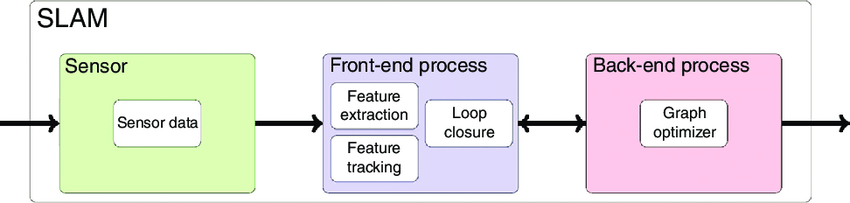
\includegraphics[width=\linewidth]{../konten/gb_slam.png}
	\caption{Basic Graph-Based SLAM Architecture \cite{ref_gb_slam}}
	\label{fig:basic_graph_based_slam}
\end{figure} 

There are three main process that can be seen from figure \ref{fig:basic_graph_based_slam}: The first process is sensor data, it means like acquiring data from sensors such as cameras, LIDAR, or IMU. The second process is front end process, The front end process is responsible for extracting features from the sensor data and finding a loop closure. The last process is back end process, the back end process is responsible for optimizing the graph to find the best estimate of the robot's trajectory and the map of the environment \cite{ref_gb_slam}.

\par
The optimization in Graph-based SLAM can be efficiently implemented using frameworks like GTSAM (Georgia Tech Smoothing and Mapping), a C++ library that applies nonlinear optimization over factor graphs. Factor graphs represent probabilistic relationships among variables such as odometry, landmarks, and sensor observations, and allow for efficient optimization of robot trajectories \cite{ref_gtsam}.

\section{RTAB-Map}
RTAB-Map (Real-Time Appearance-Based Mapping) is a graph-based SLAM framework designed for real-time applications in robotics. It integrates various sensors, including cameras, LIDARs, GPS, IMUs, and Odometry, to build a map of the environment while simultaneously localizing the robot within that map. RTAB-Map is particularly effective in large-scale environments and can handle loop closures and dynamic changes in the environment \cite{ref_rtabmap}.

\section{Stereo Depth Camera}
A stereo depth camera is a vision-based depth sensing system that uses two calibrated cameras to capture two images from slightly different perspectives—similar to human binocular vision. By analyzing the disparity between corresponding points in the image pair, the system calculates the depth or distance of objects \cite{scharstein2002taxonomy}.

\par
Stereo cameras are widely used in robotics due to their ability to generate real-time depth maps without requiring active sensors like LiDAR. They are especially useful in lightweight and power-efficient robotic platforms such as drones and small autonomous vehicles \cite{khoshelham2012accuracy}.

\section{Machine Learning}
Machine learning (ML) is a subset of artificial intelligence that focuses on creating algorithms capable of learning from data and improving performance without being explicitly programmed \cite{mitchell1997machine}. In robotics and electrical engineering, ML is essential for building intelligent systems that can recognize patterns, make decisions, and adapt to changing environments.

\par
ML methods are typically categorized into three types: supervised learning, unsupervised learning, and reinforcement learning \cite{goodfellow2016deep}. Supervised learning uses labeled datasets for tasks like classification and regression. Unsupervised learning deals with unlabeled data for clustering or dimensionality reduction. Reinforcement learning enables systems to learn optimal behaviors through reward-based interactions with the environment.

\par
A key ML technique in robotic perception is semantic segmentation, which classifies each pixel in an image into predefined categories. This technique is widely used for road detection, scene understanding, and navigation.

\section{Semantic Segmentation}

Fast-SCNN (Fast Semantic Segmentation Convolutional Neural Network) was designed for real-time performance on resource-constrained devices, making it ideal for embedded systems like autonomous vehicles. It combines a lightweight encoder-decoder structure with efficient components such as depthwise separable convolutions and a streamlined feature fusion strategy. These design choices enable Fast-SCNN to achieve a good balance between accuracy and speed, ensuring that road segmentation can be performed in real time without requiring GPU-level hardware.

\begin{figure}[H]
	\centering
	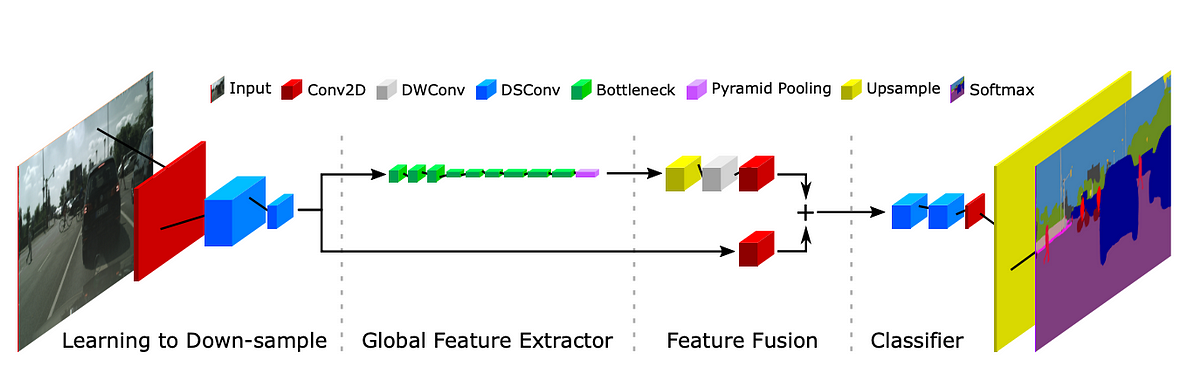
\includegraphics[width=\linewidth]{../konten/fast_scnn.png}
	\caption{Fast SCNN Architecture \cite{ref_fast_scnn}}
	\label{fig:fast_scnn_architecture}
\end{figure} 

Fast-SCNN consists of four main modules: Learning to Downsample, Global Feature Extractor, Feature Fusion Module, and Classifier. The network first reduces the spatial dimensions of the input image while increasing feature richness, then extracts global context features and fuses them with fine spatial details. This fused representation is finally classified at the pixel level to distinguish road and non-road areas. In the Icar system, this segmented output supports safe navigation by identifying drivable regions based on real-time camera input \cite{ref_fast_scnn}.

\section{Iterative Closest Point (ICP)}
Iterative Closest Point (ICP) is a widely used algorithm in known-map localization that aligns two 3D point clouds: one from the robot's current observation and one from a reference map \cite{ref_icp}. The output is a transformation matrix that minimizes the difference between the two point sets.

\par
The ICP algorithm operates in three main steps: first, for each point in the input point cloud, it finds the nearest point in the reference point cloud (using nearest-neighbor search). Second, it calculates the centroids (center of mass) of both point clouds and aligns them via translation. Third, it applies rotation—typically using Singular Value Decomposition (SVD)—to best align the clouds.

\par
These steps are repeated iteratively until convergence, defined by either reaching a maximum number of iterations or achieving a sufficiently low alignment error. The final result is the transformation matrix that aligns the current observation with the reference map, enabling accurate pose estimation.

\section{Binary Robust invariant scalable keypoints (BRISK)}
BRISK Binary Robust invariant scalable keypoints is a real-time feature method that combines a novel scale-space FAST detector with a binary bit-string descriptor built from intensity-comparison sampling. Keypoints are detected across scales via a FAST-based pyramid, then each is described by a 512-bit string derived from Gaussian-smoothed intensity comparisons on concentric sampling rings, with an orientation normalization step for rotation invariance. Evaluated on standard benchmarks, BRISK matches the accuracy of heavy float descriptors like SURF and SIFT while running up to an order of magnitude faster, making it highly suited for resource-constrained, real-time vision applications \cite{ref_brisk}.
	\cleardoublepage
	\chapter{METHODOLOGY}
\label{sec:chap3_metodologi}

\section*{ }
\section{Overview of the Icar System} 
The navigation system in Icar is divided into two types: the legacy navigation system using GNSS and the new navigation system that operates without GNSS. Below are block diagrams of Icar's navigation systems with and without GNSS.

\begin{figure}[H]
	\centering
	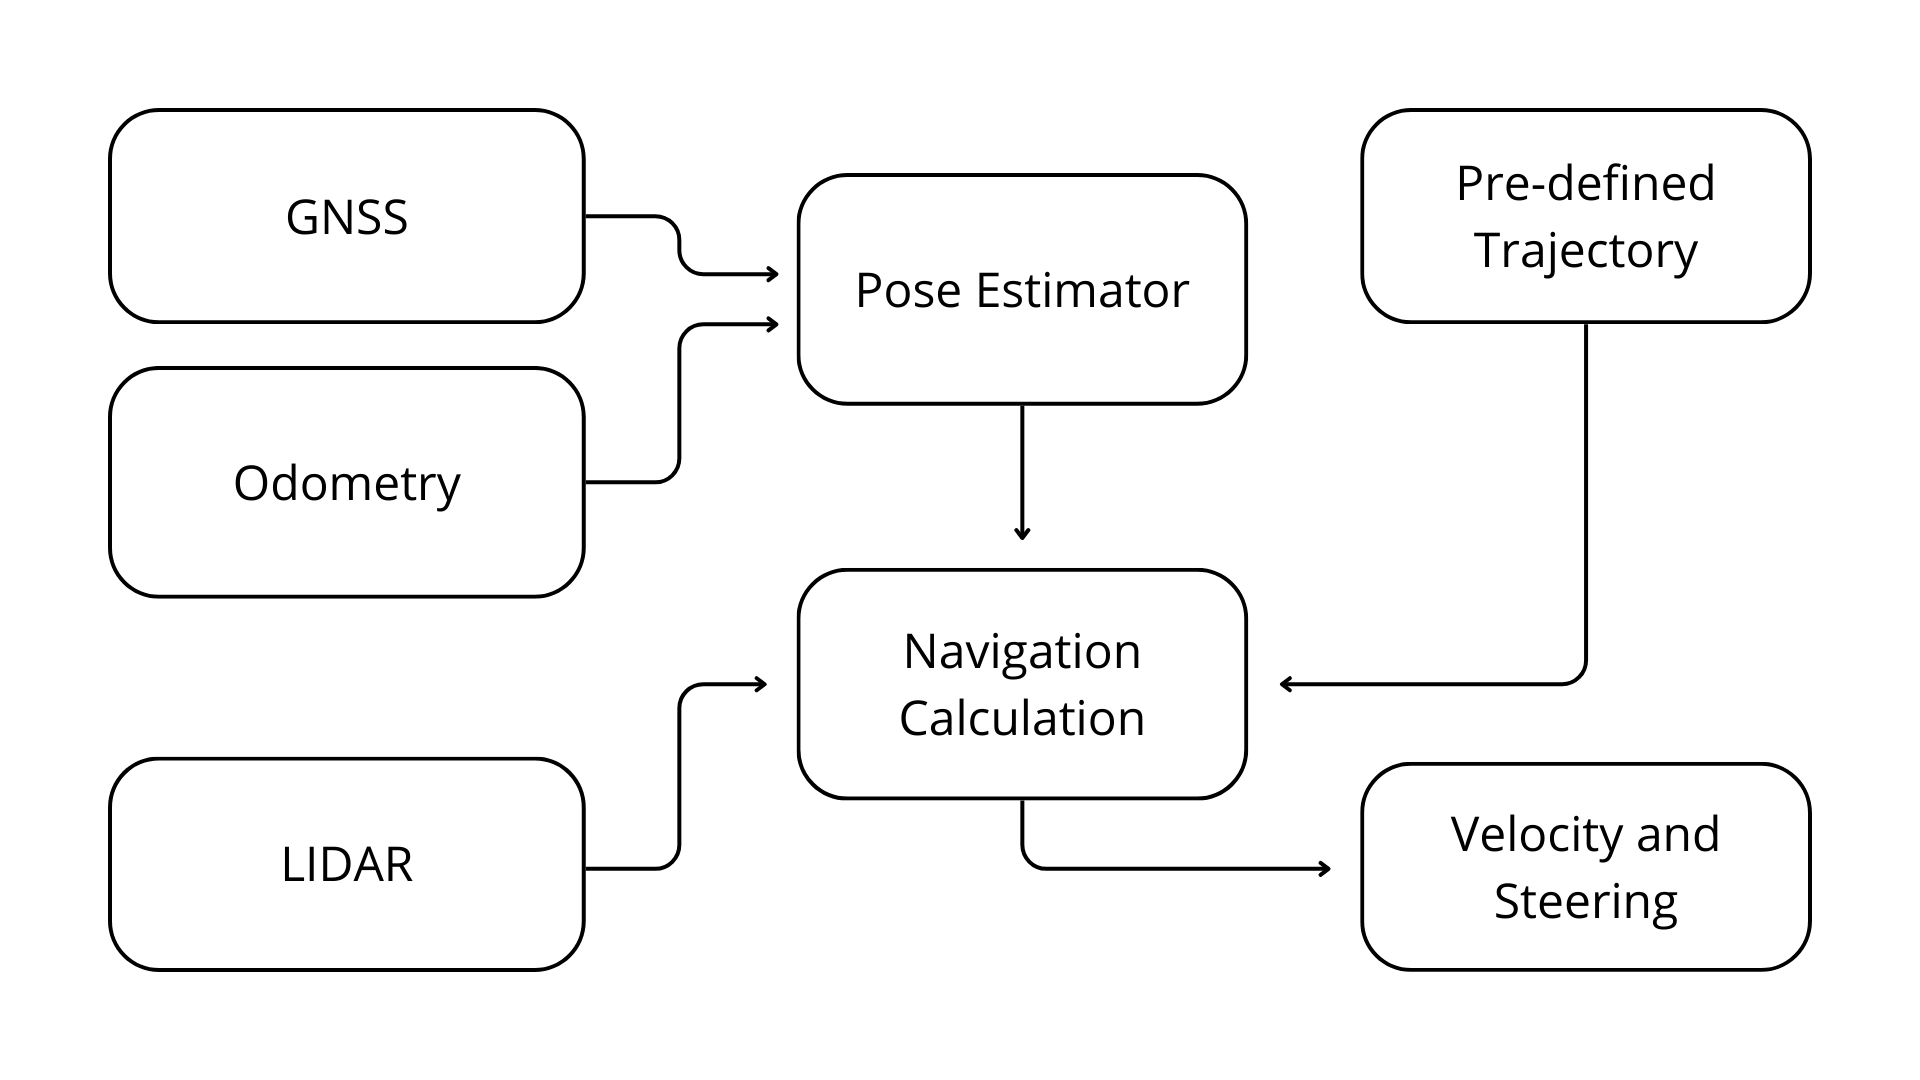
\includegraphics[width=\linewidth]{../konten/full_sys1.png}
	\caption{Block Diagram of the Legacy Icar System with GNSS}
	\label{fig:full_system}
\end{figure}
\FloatBarrier

Figure \ref{fig:full_system} illustrates the legacy Icar system, which relies on GNSS and odometry for pose estimation. The system uses a Pre-defined Trajectory to determine the target speed and steering angle using the Bicycle Model, as shown in equation~\ref{eq:bicycle_model_core}.

\begin{figure}[H]
	\centering
	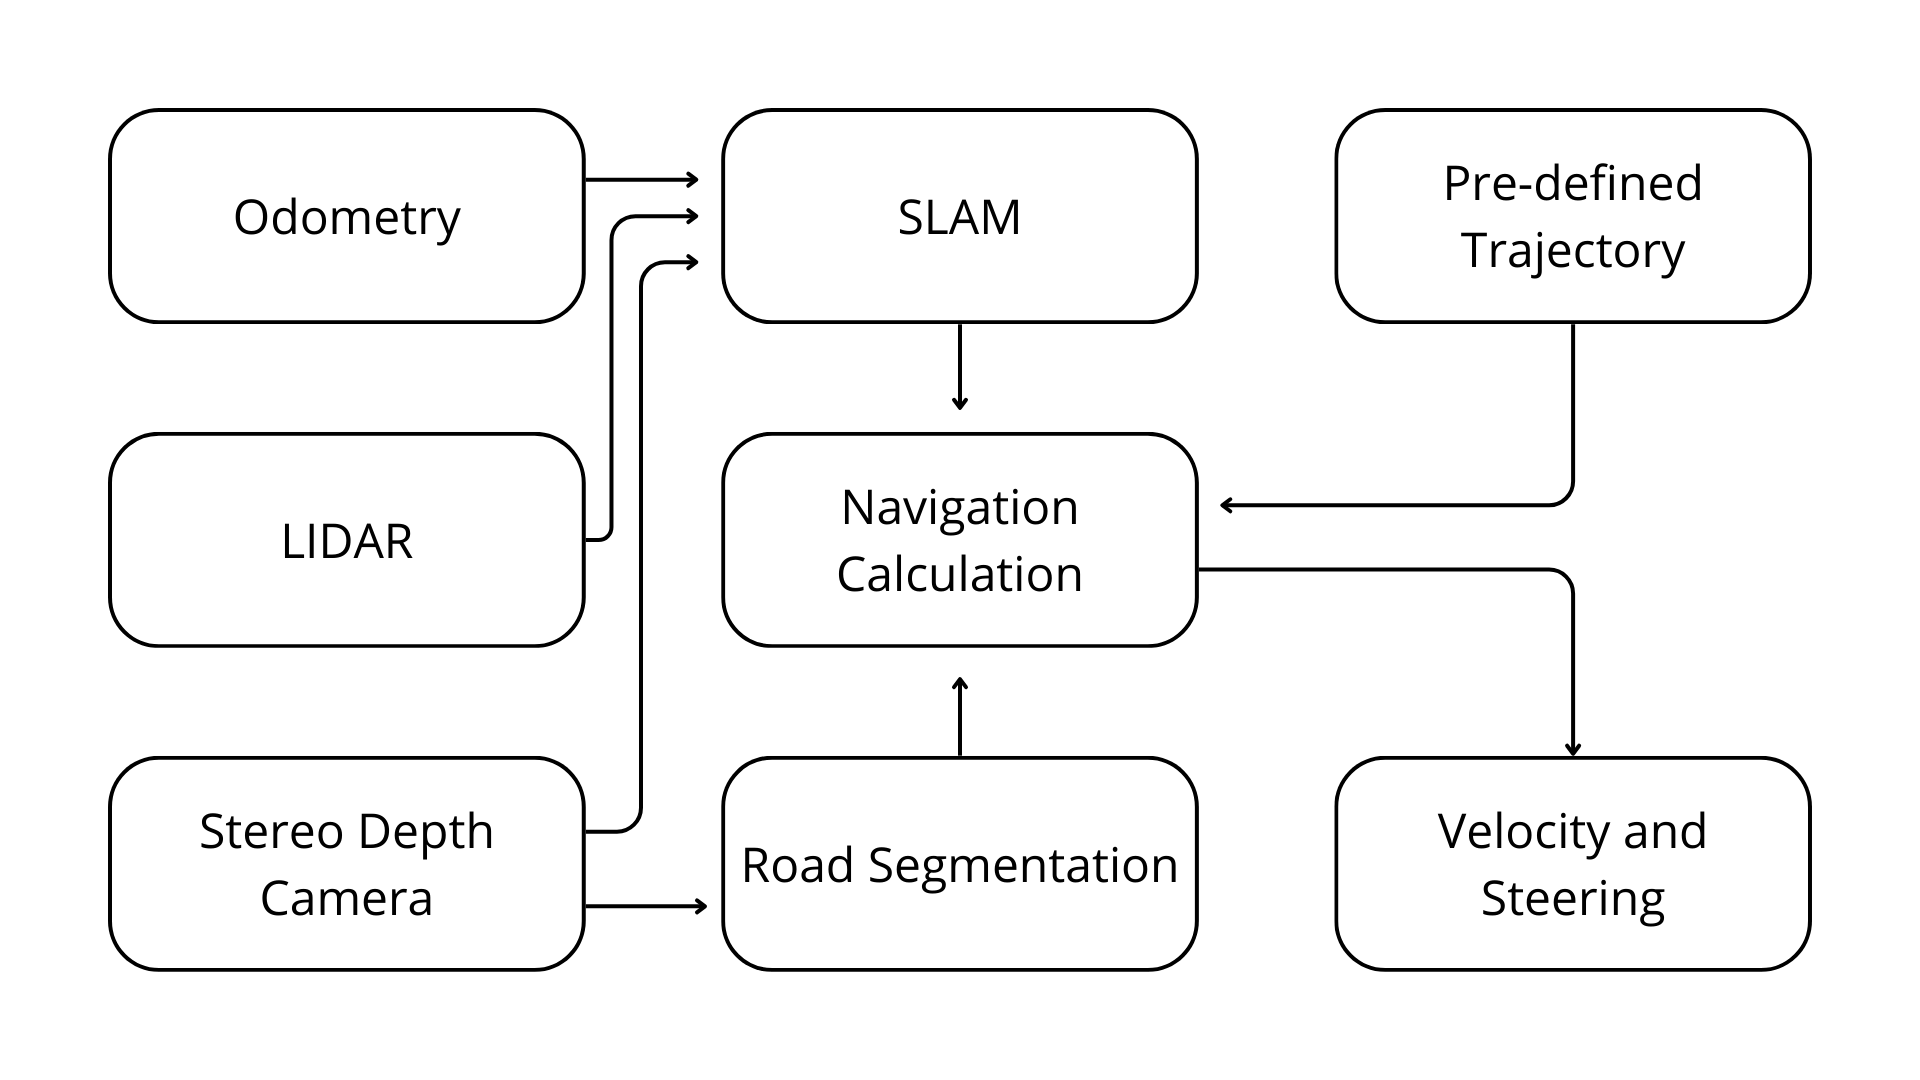
\includegraphics[width=\linewidth]{../konten/full_sys_slam1.png}
	\caption{Block Diagram of the New Icar System without GNSS}
	\label{fig:full_system_slam}
\end{figure}

Figure \ref{fig:full_system_slam} illustrates the new proposed Icar system, which does not rely on GNSS. Instead, it uses a stereo depth camera and LIDAR for pose estimation. The system also employs a Pre-defined Trajectory to determine the target speed and steering angle using the Bicycle Model, as shown in equation~\ref{eq:bicycle_model_full}. Below is the full equation for the Bicycle Model used in the new system:

\begin{equation}
	\begin{aligned}
		\Delta x &= x_{\text{waypoint}} - x_{\text{position}} \\
		\Delta y &= y_{\text{waypoint}} - y_{\text{position}} \\
		\theta_{\text{direction}} &= \tan^{-1}\left(\frac{\Delta y}{\Delta x}\right) - \theta_{\text{orientation}} \\
		v_{\text{target}} &= \min\left(\sqrt{\Delta x^2 + \Delta y^2}, \ v_{\text{max}}\right) \\
		\delta_{\text{target}} &= \tan^{-1}\left( \frac{2 \cdot L \cdot \sin(\theta_{\text{direction}})}{D_{\text{lookahead}}} \right)
		\label{eq:bicycle_model_full}
	\end{aligned}		
\end{equation}

Where $x_{\text{waypoint}}$ and $y_{\text{waypoint}}$ are the coordinates of the waypoint obtained from the Pre-defined Trajectory, $x_{\text{position}}$ and $y_{\text{position}}$ represent the vehicle's current position, $\theta_{\text{direction}}$ is the heading angle, $\theta_{\text{orientation}}$ is the current orientation, $v_{\text{target}}$ is the target velocity, $v_{\text{max}}$ is the maximum velocity, $\delta_{\text{target}}$ is the target steering angle, $L$ is the distance between the front and rear wheels, and $D_{\text{lookahead}}$ is the lookahead distance.

The primary difference between the two systems is the source of position and orientation data. The legacy system uses GNSS and odometry, while the new system uses stereo depth cameras, LIDAR, and odometry. Additionally, the new system integrates road detection to enhance navigation safety.

\section{Road Detection System}
\begin{figure}[H]
	\centering
	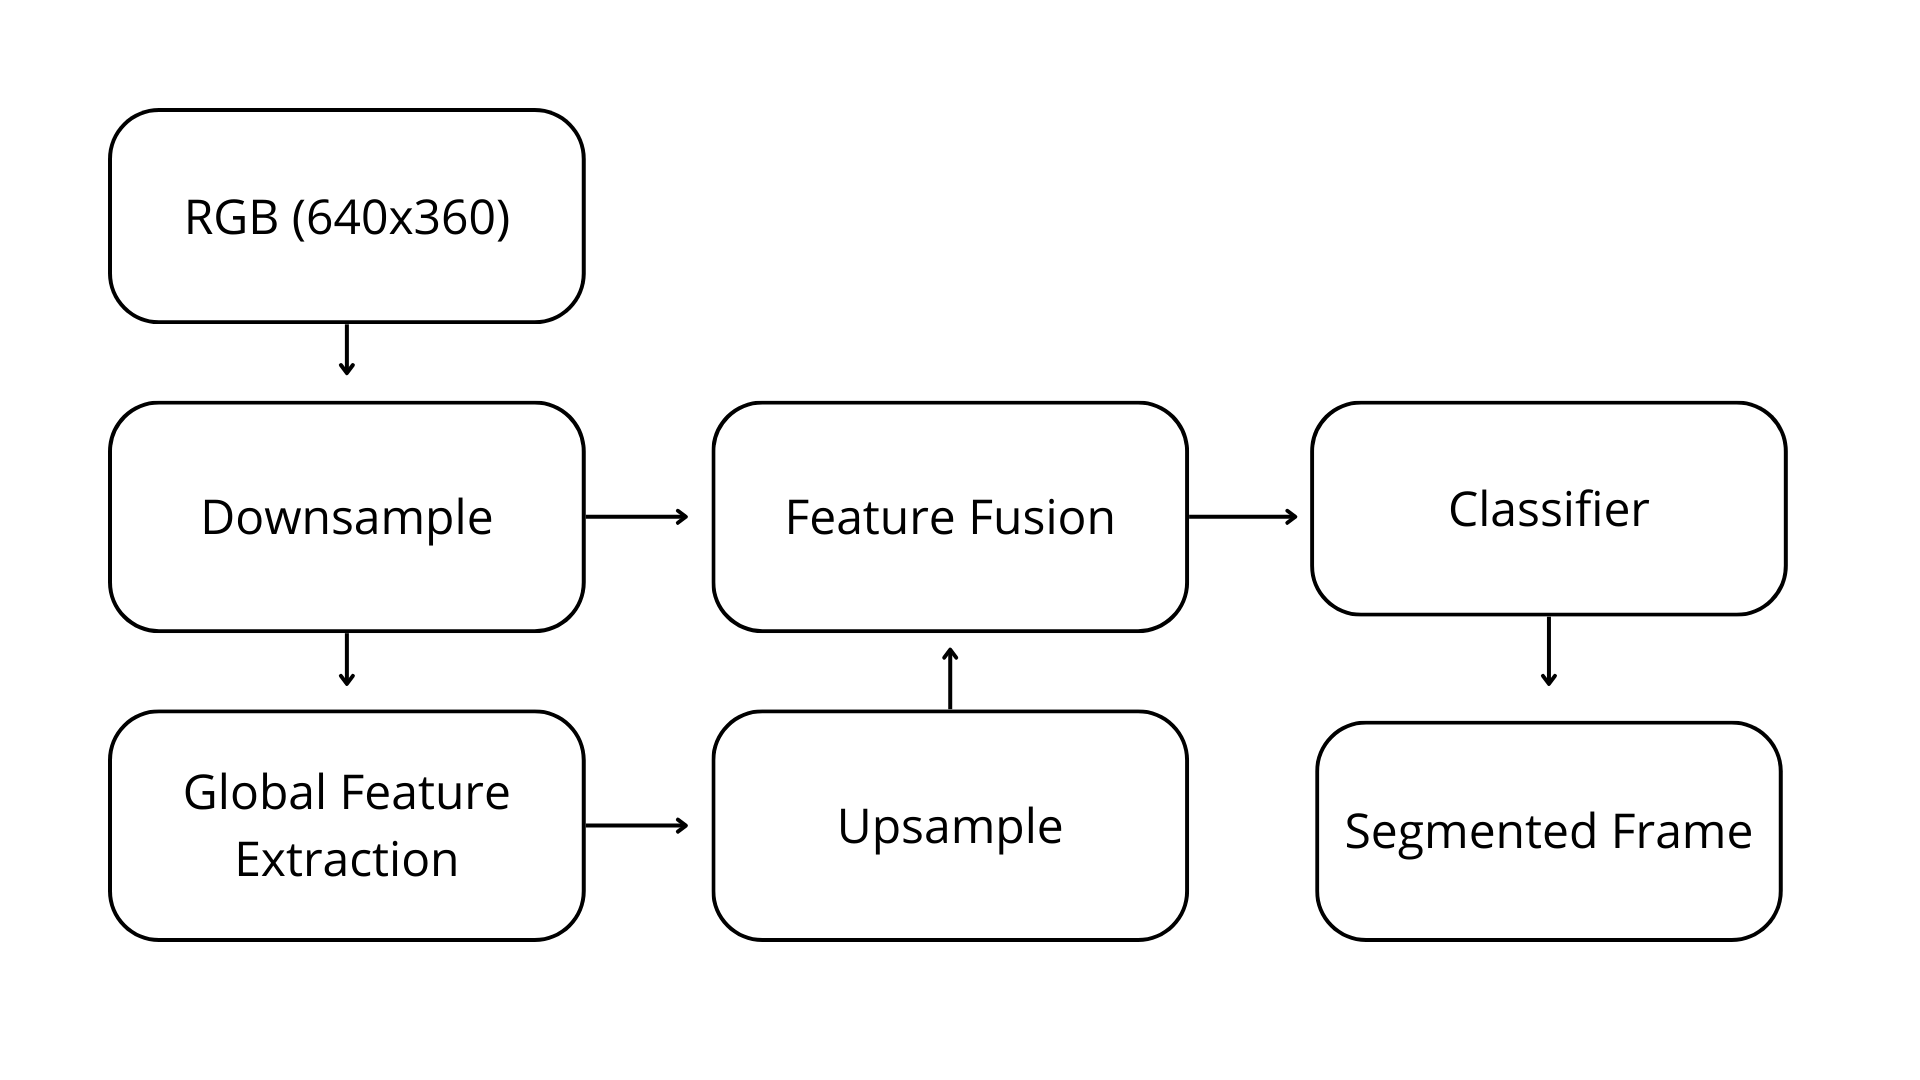
\includegraphics[width=\linewidth]{../konten/ml_sys.png}
	\caption{Block Diagram of the Machine Learning Architecture on Icar}
	\label{fig:ml_system}
\end{figure} 

From Figure \ref{fig:ml_system}, it is shown that the road detection system on Icar utilizes a machine learning architecture, specifically using Fast-SCNN \cite{ref_fast_scnn} as the core model. Its architecture differs in the convolution channels and pooling methods. The smaller convolution channels and the use of average pooling instead of pyramid pooling are intended to reduce computational load, making it suitable for real-time applications on Icar.

\subsection{Downsampling} 
In this step, the image captured by the stereo depth camera, originally a 3-channel image, is converted to 16 channels. This is achieved via three successive 3x3 convolution layers with a stride of 2: first converting 3→4 channels, then 4→8, and finally 8→16 channels. The resulting image is then split into two paths: one goes to global feature extraction, the other to feature fusion.

\subsection{Global Feature Extraction}
This stage performs a depthwise-separable convolution to extract features from the 16-channel image. This method is chosen for its computational efficiency. The result is a 24-channel image, which is passed on to the upsampling stage.

\subsection{Upsampling}
This step performs pooling using average pooling, which is lighter and faster compared to the pyramid pooling used in the original Fast-SCNN. A convolution then produces a 32-channel output, which is passed to feature fusion.

\subsection{Feature Fusion}
Here, outputs from the downsampling and global feature extraction stages are merged into a 48-channel image. Before merging, image dimensions are matched using bilinear interpolation. The merged result is passed to the classification stage.

\subsection{Classification}
In this final stage, the 48-channel image undergoes classification using ReLU, producing a 2-channel image indicating road and non-road areas. This image then proceeds to post processing.

\section{Pose and Orientation Correction System}
\begin{figure}[H]
	\centering
	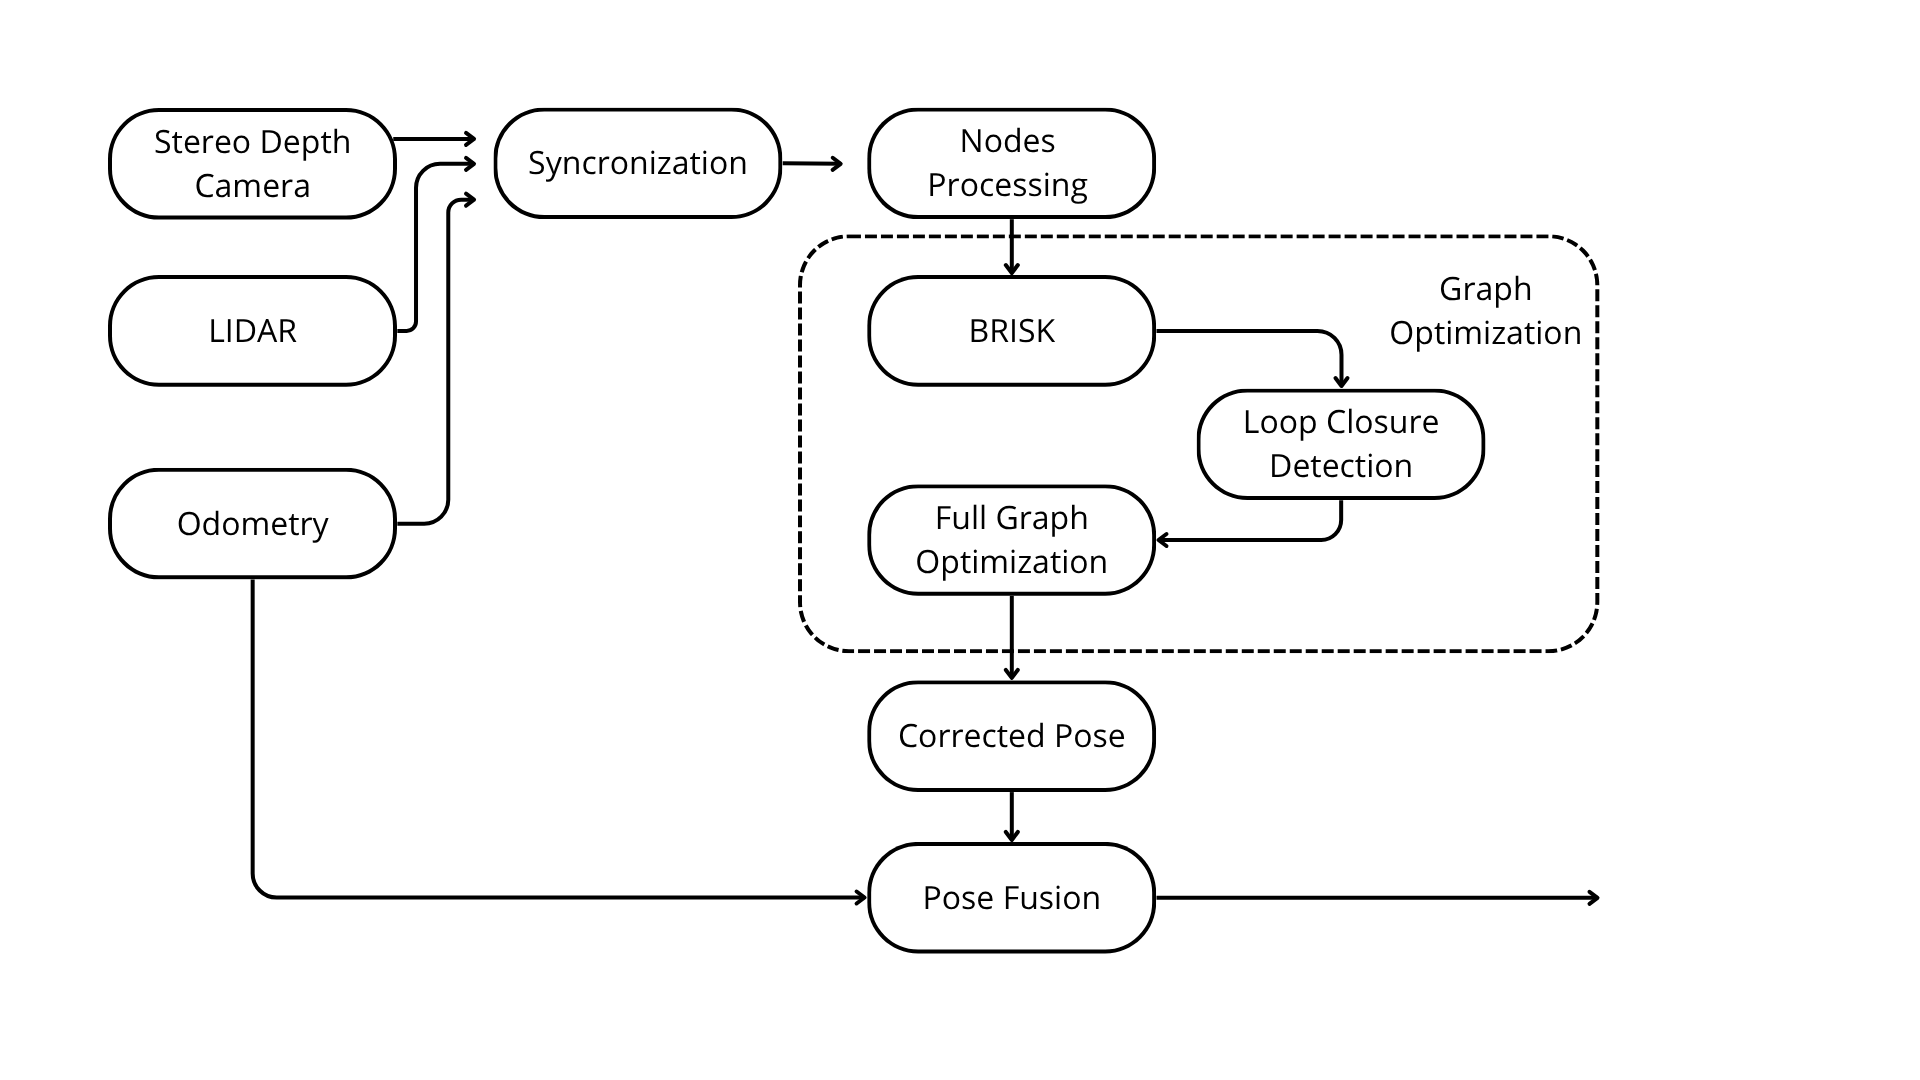
\includegraphics[width=\linewidth]{../konten/GNSS(20).png}
	\caption{Block Diagram of Pose and Orientation Correction System on Icar}
	\label{fig:slam_system}
\end{figure} 

From Figure \ref{fig:slam_system}, the pose correction system consists of four main processes: data synchronization, nodes processing, graph optimization, and pose fusion.

\subsection{Data Synchronization} 
This initial step synchronizes data from the stereo depth camera and odometry based on timestamps to ensure aligned data for further processing.

\subsection{Nodes Processing}
This initiates the graph optimization process. Nodes represent vehicle poses and keypoints from stereo depth camera and LIDAR. There are two modes:
- In mapping mode, new nodes are continuously added.
- In localization mode, existing nodes are used without adding new ones.

\subsection{Graph Optimization} 
This is the core component, using the GTSAM library. It starts finding loop closure by detecting revisited nodes, which are nodes that have been previously visited by the vehicle. The algorithm to do image matching is using BRISK. After the hypothesis of loop closure has gained, the next step is doing a full graph optimization using GTSAM, the GTSAM will minimize the error between the current pose and the previous pose, as well as the error between the current pose and the loop closure hypothesis. The result is a corrected pose of the vehicle.

\subsection{Pose Fusion} 
The final step combines poses from graph optimization and odometry using a Kalman Filter, resulting in more accurate pose estimation than using odometry alone. Using the differential data from Odometry (Wheel encoder and IMU) combined with estimated pose that coming from Graph Optimization, the system can correct the pose and orientation of Icar.

\section{Icar Navigation System with Road Detection and Graph-Based SLAM} 
\begin{figure}[H]
	\centering
	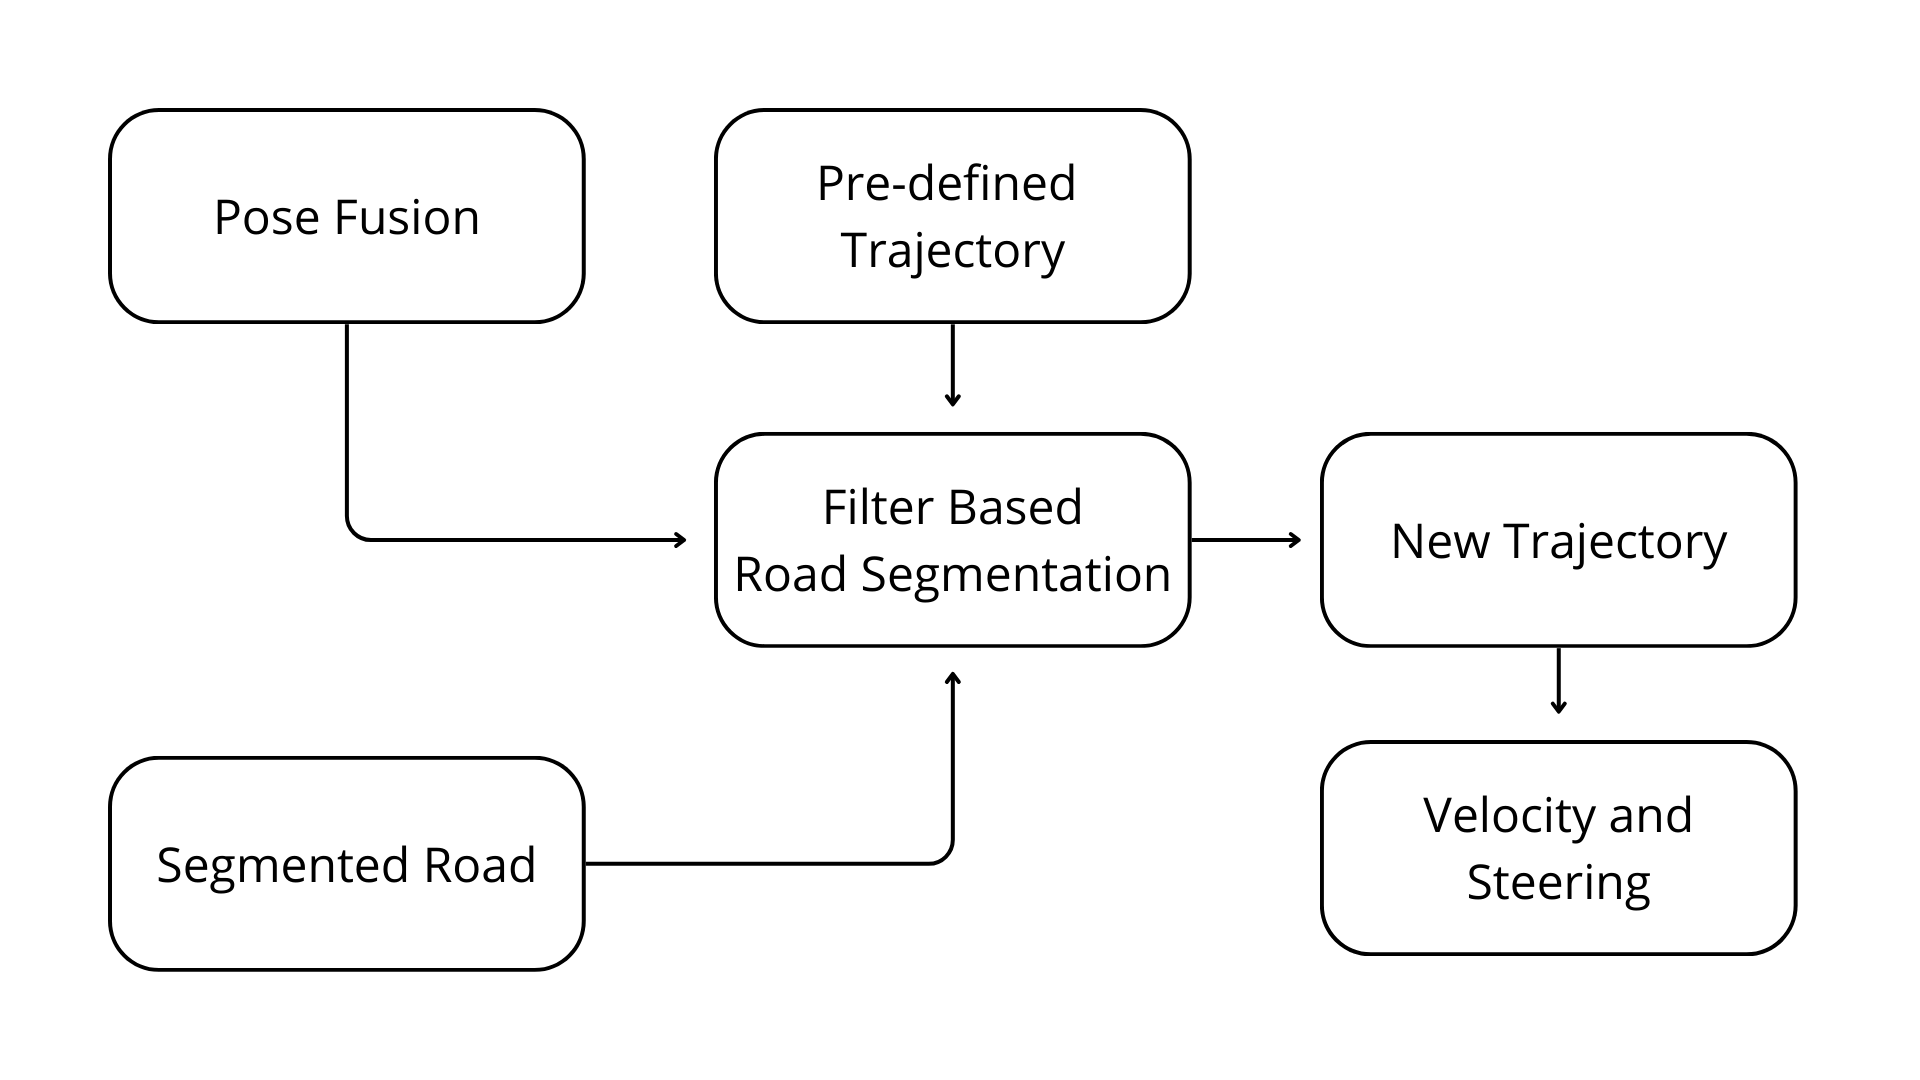
\includegraphics[width=\linewidth]{../konten/nav_new_sys3.png}
	\caption{Block Diagram of Icar Navigation System with Road Detection and Graph-Based SLAM}
	\label{fig:nav_new_system}
\end{figure} 

This diagram expands upon Figure \ref{fig:full_system_slam}, showing how the segmented road image from Figure \ref{fig:ml_system} and the pose data from Figure \ref{fig:slam_system} are integrated into a unified and improved navigation system.

\par  
The first step selects waypoints based on current pose (from graph-based SLAM) and the pre-defined trajectory. These waypoints are overlaid on the road segmentation image.

\par   
Next, a check is performed using a bitwise AND operation to determine if all waypoints lie within the road area. If so, the selected waypoints are used as the new trajectory.

\par  
If any waypoint lies outside the road, a new trajectory is generated using the image’s center of mass, converted into vehicle coordinates. A straight line is then created from the current position to the center of mass.

\par 
This new trajectory is then used for vehicle navigation. The vehicle follows it using the Bicycle Model as defined in Equation \ref{eq:bicycle_model_full} to calculate target speed and steering angle.

	\cleardoublepage
	\chapter{RESEARCH PLAN}
% Please add the following required packages to your document preamble:
% \usepackage{multirow}
% \usepackage[table,xcdraw]{xcolor}
% If you use beamer only pass "xcolor=table" option, i.e. \documentclass[xcolor=table]{beamer}
\begin{table*}[h]
	\centering
	\caption{Research Schedule}
	\begin{tabular}{|l|llllllllllllllll|}
		\hline
		\multicolumn{1}{|c|}{}                                                             & \multicolumn{16}{c|}{Weeks-} \\ \cline{2-17} 
		\multicolumn{1}{|c|}{\multirow{-2}{*}{Activities}}                                   & \multicolumn{1}{l|}{1}                        & \multicolumn{1}{l|}{2}                        & \multicolumn{1}{l|}{3}                        & \multicolumn{1}{l|}{4}                        & \multicolumn{1}{l|}{5}                        & \multicolumn{1}{l|}{6}                        & \multicolumn{1}{l|}{7}                        & \multicolumn{1}{l|}{8}                        & \multicolumn{1}{l|}{9}                        & \multicolumn{1}{l|}{10}                       & \multicolumn{1}{l|}{11}                       & \multicolumn{1}{l|}{12}                       & \multicolumn{1}{l|}{13}                       & \multicolumn{1}{l|}{14}                       & \multicolumn{1}{l|}{15}                       & 16                       \\ \hline
		\begin{tabular}[c]{@{}l@{}}Literature \\ Study\end{tabular}                             & \multicolumn{1}{l|}{\cellcolor[HTML]{F8FF00}} & \multicolumn{1}{l|}{\cellcolor[HTML]{F8FF00}} & \multicolumn{1}{l|}{}                         & \multicolumn{1}{l|}{}                         & \multicolumn{1}{l|}{}                         & \multicolumn{1}{l|}{}                         & \multicolumn{1}{l|}{}                         & \multicolumn{1}{l|}{}                         & \multicolumn{1}{l|}{}                         & \multicolumn{1}{l|}{}                         & \multicolumn{1}{l|}{}                         & \multicolumn{1}{l|}{}                         & \multicolumn{1}{l|}{}                         & \multicolumn{1}{l|}{}                         & \multicolumn{1}{l|}{}                         &                          \\ \hline
		\begin{tabular}[c]{@{}l@{}}Road \\ Image \\ Dataset \\ Creation\\\end{tabular}                  & \multicolumn{1}{l|}{}                         & \multicolumn{1}{l|}{}                         & \multicolumn{1}{l|}{\cellcolor[HTML]{F8FF00}} & \multicolumn{1}{l|}{}                         & \multicolumn{1}{l|}{}                         & \multicolumn{1}{l|}{}                         & \multicolumn{1}{l|}{}                         & \multicolumn{1}{l|}{}                         & \multicolumn{1}{l|}{}                         & \multicolumn{1}{l|}{}                         & \multicolumn{1}{l|}{}                         & \multicolumn{1}{l|}{}                         & \multicolumn{1}{l|}{}                         & \multicolumn{1}{l|}{}                         & \multicolumn{1}{l|}{}                         &                          \\ \hline
		\begin{tabular}[c]{@{}l@{}}Road \\ Segmen-\\tation \\ Training \\ and Test\end{tabular}       & \multicolumn{1}{l|}{}                         & \multicolumn{1}{l|}{}                         & \multicolumn{1}{l|}{\cellcolor[HTML]{F8FF00}} & \multicolumn{1}{l|}{\cellcolor[HTML]{F8FF00}} & \multicolumn{1}{l|}{\cellcolor[HTML]{F8FF00}} & \multicolumn{1}{l|}{}                         & \multicolumn{1}{l|}{}                         & \multicolumn{1}{l|}{}                         & \multicolumn{1}{l|}{}                         & \multicolumn{1}{l|}{}                         & \multicolumn{1}{l|}{}                         & \multicolumn{1}{l|}{}                         & \multicolumn{1}{l|}{}                         & \multicolumn{1}{l|}{}                         & \multicolumn{1}{l|}{}                         &                          \\ \hline
		\begin{tabular}[c]{@{}l@{}}Map \\ Creation \\ for SLAM\end{tabular} & \multicolumn{1}{l|}{}                         & \multicolumn{1}{l|}{}                         & \multicolumn{1}{l|}{}                         & \multicolumn{1}{l|}{}                         & \multicolumn{1}{l|}{\cellcolor[HTML]{F8FF00}} & \multicolumn{1}{l|}{\cellcolor[HTML]{F8FF00}} & \multicolumn{1}{l|}{\cellcolor[HTML]{F8FF00}} & \multicolumn{1}{l|}{}                         & \multicolumn{1}{l|}{}                         & \multicolumn{1}{l|}{}                         & \multicolumn{1}{l|}{}                         & \multicolumn{1}{l|}{}                         & \multicolumn{1}{l|}{}                         & \multicolumn{1}{l|}{}                         & \multicolumn{1}{l|}{}                         &                          \\ \hline

		\begin{tabular}[c]{@{}l@{}}End to \\ End Test\end{tabular}                 & \multicolumn{1}{l|}{}                         & \multicolumn{1}{l|}{}                         & \multicolumn{1}{l|}{}                         & \multicolumn{1}{l|}{}                         & \multicolumn{1}{l|}{}                         & \multicolumn{1}{l|}{}                         & \multicolumn{1}{l|}{\cellcolor[HTML]{F8FF00}} & \multicolumn{1}{l|}{\cellcolor[HTML]{F8FF00}} & \multicolumn{1}{l|}{\cellcolor[HTML]{F8FF00}} & \multicolumn{1}{l|}{\cellcolor[HTML]{F8FF00}} & \multicolumn{1}{l|}{\cellcolor[HTML]{F8FF00}} & \multicolumn{1}{l|}{\cellcolor[HTML]{F8FF00}} & \multicolumn{1}{l|}{\cellcolor[HTML]{F8FF00}}                         & \multicolumn{1}{l|}{\cellcolor[HTML]{F8FF00}}                         & \multicolumn{1}{l|}{\cellcolor[HTML]{F8FF00}}                         & \multicolumn{1}{l|}{\cellcolor[HTML]{F8FF00}}                         \\ \hline

		Analysis                                                                            & \multicolumn{1}{l|}{}                         & \multicolumn{1}{l|}{}                         & \multicolumn{1}{l|}{}                         & \multicolumn{1}{l|}{}                         & \multicolumn{1}{l|}{}                         & \multicolumn{1}{l|}{}                         & \multicolumn{1}{l|}{\cellcolor[HTML]{F8FF00}} & \multicolumn{1}{l|}{\cellcolor[HTML]{F8FF00}} & \multicolumn{1}{l|}{\cellcolor[HTML]{F8FF00}} & \multicolumn{1}{l|}{\cellcolor[HTML]{F8FF00}} & \multicolumn{1}{l|}{\cellcolor[HTML]{F8FF00}} & \multicolumn{1}{l|}{\cellcolor[HTML]{F8FF00}} & \multicolumn{1}{l|}{\cellcolor[HTML]{F8FF00}}                         & \multicolumn{1}{l|}{\cellcolor[HTML]{F8FF00}}                         & \multicolumn{1}{l|}{\cellcolor[HTML]{F8FF00}}                         & \multicolumn{1}{l|}{\cellcolor[HTML]{F8FF00}}                         \\ \hline
		

		% \begin{tabular}[c]{@{}l@{}}Publication \\ Process\end{tabular}                                                   & \multicolumn{1}{l|}{}                         & \multicolumn{1}{l|}{}                         & \multicolumn{1}{l|}{}                         & \multicolumn{1}{l|}{}                         & \multicolumn{1}{l|}{}                         & \multicolumn{1}{l|}{}                         & \multicolumn{1}{l|}{}                         & \multicolumn{1}{l|}{}                         & \multicolumn{1}{l|}{}                         & \multicolumn{1}{l|}{}                         & \multicolumn{1}{l|}{}                         & \multicolumn{1}{l|}{\cellcolor[HTML]{F8FF00}} & \multicolumn{1}{l|}{\cellcolor[HTML]{F8FF00}} & \multicolumn{1}{l|}{\cellcolor[HTML]{F8FF00}} & \multicolumn{1}{l|}{\cellcolor[HTML]{F8FF00}} & \cellcolor[HTML]{F8FF00} \\ \hline
	\end{tabular}
\end{table*}
	\cleardoublepage
	%\chapter{PENUTUP}
\label{sec:chap5_tutup}
\vspace{1ex}
\section*{}
Setelah penerapan metode terhadap masalah yang ingin diselesaikan pada \vspace{1ex}

\section{Kesimpulan}
\label{sec:sec4_kesimpulan}
\vspace{1ex}
\lipsum[1]
\section{Saran}
\label{sec:sec4_saran}
\vspace{1ex}
\lipsum[2]


	%\cleardoublepage
	%Bab Lain bisa ditambah disini
\end{spacing}
\DaftarPustaka
% Daftar Riwayat Hidup
%    ->\ubah\DaftarRiwayatHidup.tex
\DaftarRiwayatHidup
\end{document}